\documentclass{article}
%\usepackage[english]{babel}%
\usepackage{graphicx}
\usepackage{tabulary}
\usepackage{tabularx}
\usepackage[table,xcdraw]{xcolor}
\usepackage{pdflscape}
%\usepackage{gensymb}
\usepackage{lastpage}
\usepackage{multirow}
\usepackage{xcolor}
\usepackage{cancel}
\usepackage{amsmath}
\usepackage[table]{xcolor}
\usepackage{fixltx2e}
\usepackage[T1]{fontenc}
\usepackage[utf8]{inputenc}
\usepackage{ifthen}
\usepackage{fancyhdr}
\usepackage[utf8]{inputenc}
\usepackage{tikz}
\usepackage[document]{ragged2e}
\usepackage[margin=1 in,top=1.2in,headheight=57pt,headsep=0.1in]
{geometry}
\usepackage{ifthen}
\usepackage{fancyhdr}
\everymath{\displaystyle}
\usepackage[document]{ragged2e}
\usepackage{fancyhdr}
\usepackage{mathabx}
\usepackage{textcomp,mathcomp}
\usepackage[shortlabels]{enumitem}
\everymath{\displaystyle}
\linespread{2}%controls the spacing between lines. Bigger fractions means crowded lines%
\linespread{1.3}%controls the spacing between lines. Bigger fractions means crowded lines%
\pagestyle{fancy}
\setlength{\headheight}{56.2pt}
\usepackage{soul}
\usepackage{siunitx}

%\usepackage{textcomp}
\usetikzlibrary{shapes.multipart, shapes.geometric, arrows}
\usetikzlibrary{calc, decorations.markings}
\usetikzlibrary{arrows.meta}
\usetikzlibrary{shapes,snakes}
\usetikzlibrary{quotes,angles, positioning}
%\chead{\ifthenelse{\value{page}=1}{
\includegraphics[scale=0.3]{BassettCTCLogo}}}
%\rhead{\ifthenelse{\value{page}=1}{Final Exam}{}}
%\lhead{\ifthenelse{\value{page}=1}{Water Treatment - Oct-Dec 2022}{\textbf Final Exam}}
%\rfoot{\ifthenelse{\value{page}=1}{}{}}
%
%\cfoot{}
%\lfoot{Page \thepage\ of \pageref{LastPage}}
%\renewcommand{\headrulewidth}{2pt}
%\renewcommand{\footrulewidth}{1pt}
\graphicspath{ {./images/} }
\begin{document}

\begin{enumerate}
\item What is the pressure at the bottom of the reservoir when the water level is 40'?

$40 \mathrm{ft} \times 0.433 \mathrm{psi} / \mathrm{ft}=17.3 \mathrm{psi}$

\vspace{0.4cm}

\item Find the height of water in a tank if the pressure at the bottom of the tank is 12 psi.

$12 \mathrm{psi} \div 0.433 \mathrm{psi} / \mathrm{ft}=27.7 \mathrm{ft}$\\

\vspace{0.3cm}

\item 1 MGD is pumped against a 14’ head.  What is the water Hp?  The pump mechanical efficiency is 85\%.  What is the brake horsepower?\\
\vspace{0.4cm}
\vspace{0.4cm}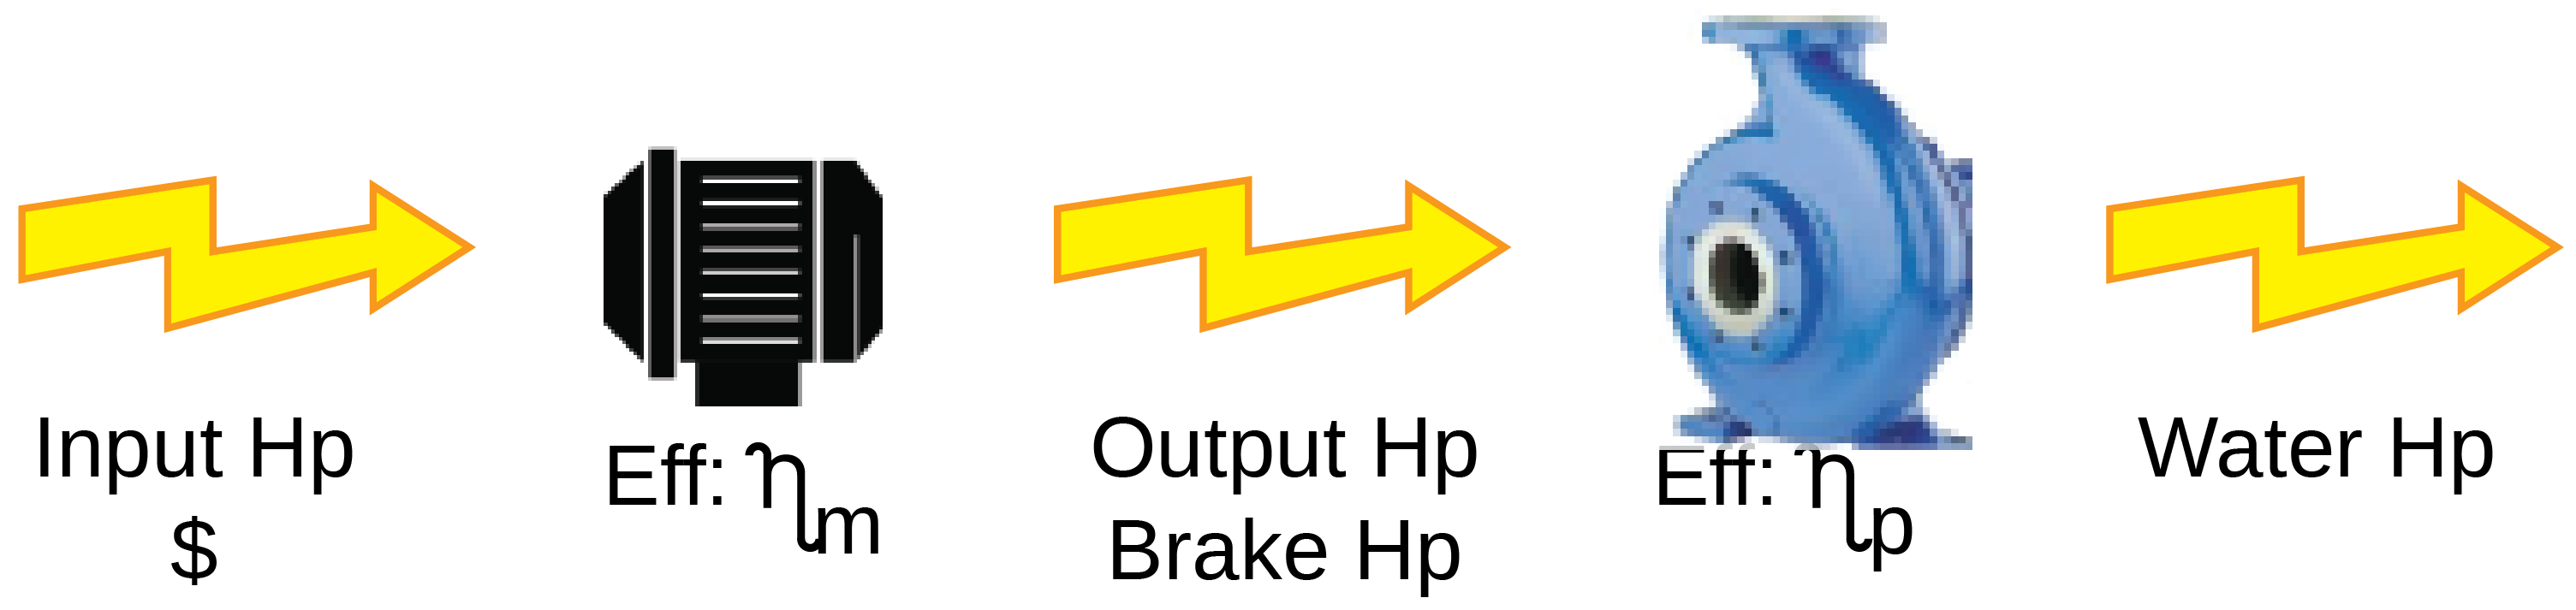
\includegraphics[scale=0.08]{PumpProblem}\\
\vspace{0.2cm}
water Hp = flow * head\\
\vspace{0.4cm}
$\dfrac{1,000,000 \enspace gal}{day}*\dfrac{day}{1440 \enspace min}*14 \enspace ft*\dfrac{Hp}{3,960 \enspace GPM-ft}=\boxed{Water \enspace Hp = 2.46 \enspace Hp}$\\
\vspace{0.4cm}
pump Hp = brake Hp * pump efficiency\\
\vspace{0.4cm}
$Brake \enspace Hp = \dfrac{2.46}{0.85}=\boxed{Brake \enspace Hp=2.89Hp}$\\
\vspace{0.4cm}

\item The water horsepower of a well with a submersible pump has been calculated at 8.2 WHp. The Output of the electric motor is measured as $10.3 \mathrm{BHp}$. What is the efficiency of the pump?\\
  \vspace{0.2cm}
 \vspace{0.08cm}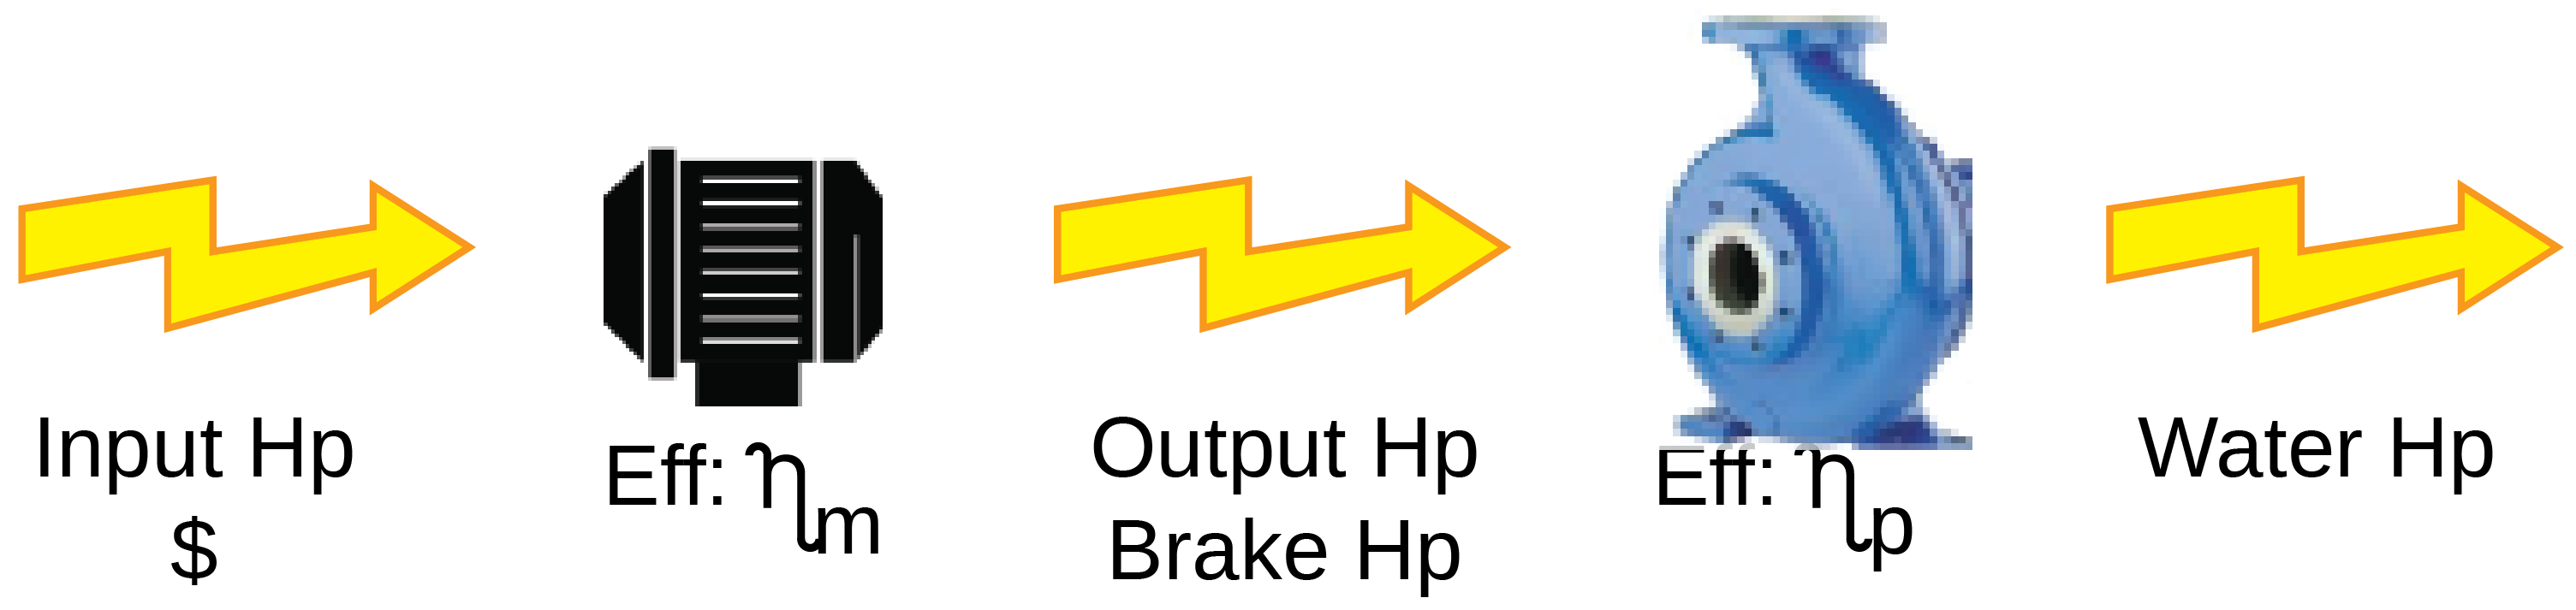
\includegraphics[scale=0.08]{PumpProblem}\\
 \vspace{0.2cm}
$\eta_p=\dfrac{8.2 \mathrm{\enspace W \enspace Hp}}{10.3 \mathrm{\enspace BHp}} \times 100=\boxed{80 \%}$
 \vspace{0.2cm}


\newpage
\item A flow of 200 GPM  is pumped against a total head of 4.0 feet. The pump is 78\% efficient and the motor is 90\% efficient. Calculate the input Hp.\\
\vspace{0.4cm}
water Hp = flow * head\\
\vspace{0.2cm}
$200GPM*4ft*\dfrac{Hp}{3,960 GPM-ft}=0.2Hp$\\
\vspace{0.4cm}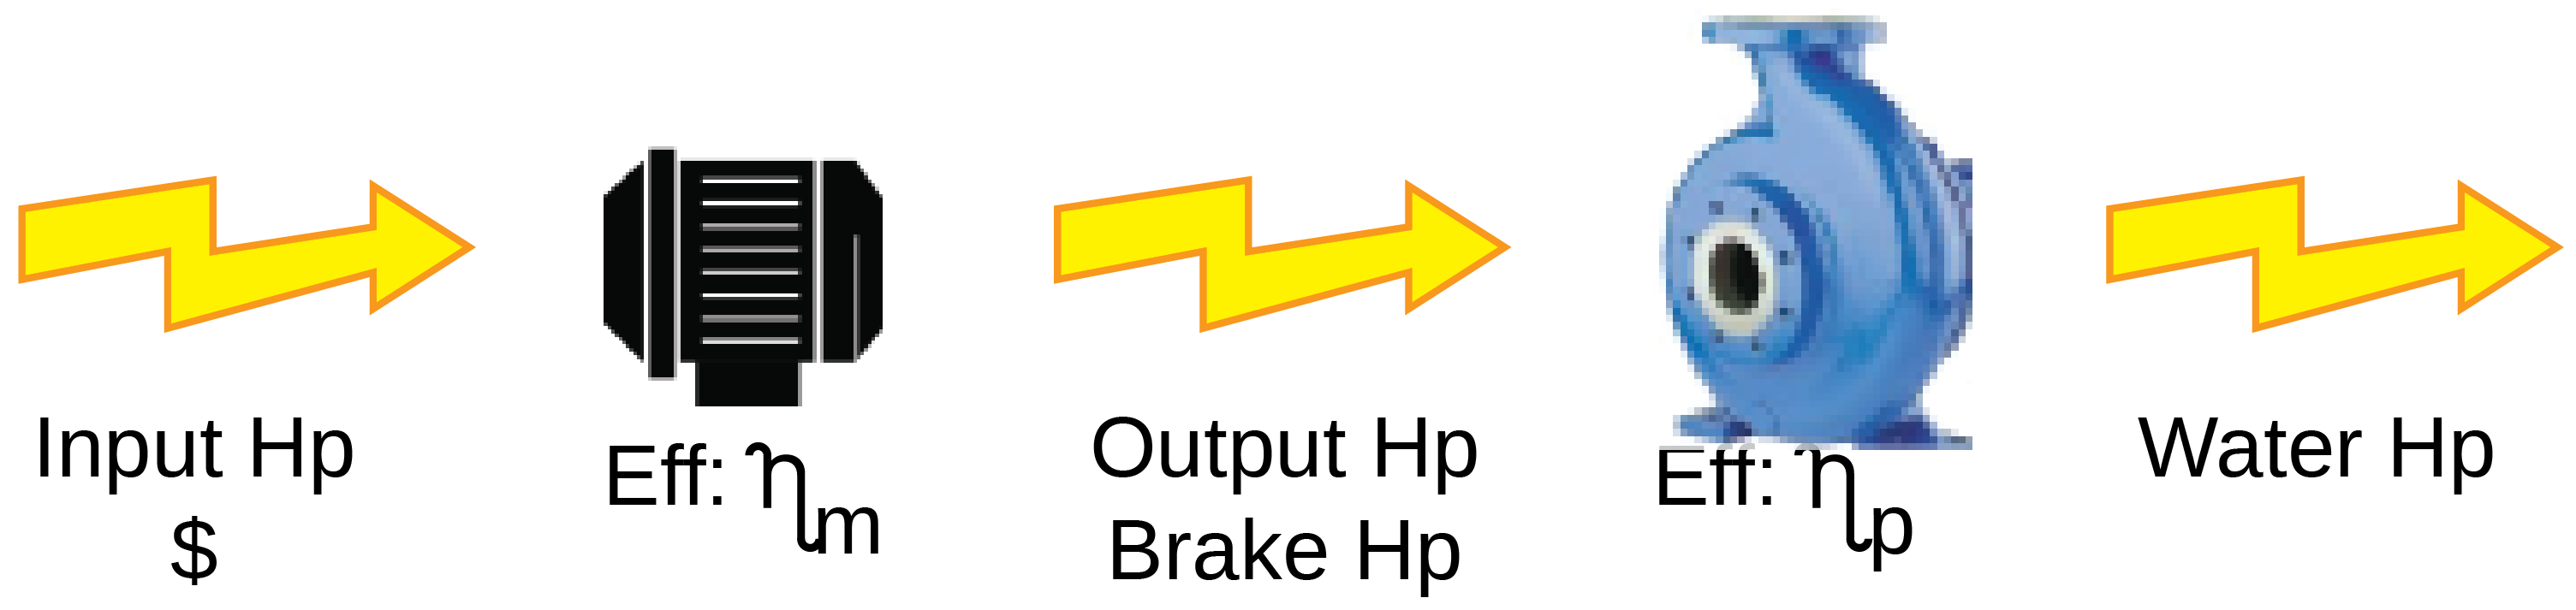
\includegraphics[scale=0.08]{PumpProblem}\\
water Hp=brake Hp*pump efficiency, and\\
brake Hp=input Hp*motor efficiency\\
Therefore, water Hp=input Hp*motor efficiency*pump efficiency\\
\vspace{0.4cm}
input Hp=$\dfrac{water \enspace Hp}{motor \enspace efficiency*pump \enspace efficiency}=\dfrac{0.2}{0.9*0.78}=\boxed{0.28Hp}$
\vspace{0.2cm}

\item 500,000 GPD of secondary effluent is pumped to  a  storage  pond  for  reuse  as golf course irrigation water.  The water is lifted 12 feet in the plant, and then pumped up another 75 feet to the storage pond. Friction losses are assumed to be 10\% of the static head.  Assuming the pump efficiency of 70\% and a motor efficiency of 92\% and an electrical cost of \$0.0725 per KWh, calculate the daily cost of pumping this water.\\
\vspace{0.4cm}
Solution:\\

water Hp = flow * head\\
\vspace{0.4cm}
$\frac{500,000gal}{day}*\frac{day}{1440min}*(87ft-static \enspace head+87*0.1ft-friction \enspace head)*\frac{Hp}{3,960 GPM-ft}$\\
\vspace{0.4cm}
$=8.39 - water \enspace Hp$\\
\vspace{0.4cm}
input Hp=$\frac{water \enspace Hp}{motor \enspace efficiency*pump \enspace efficiency}=\frac{8.39}{0.92*0.70}=\boxed{13Hp}$\\
\vspace{0.4cm}
Electrical cost=$13Hp*\frac{0.746kW}{Hp}*\frac{24hrs}{day}*\frac{\$0.0725}{kWh}=\boxed{\frac{\$16.87}{day}}$

\vspace{0.4cm}


\end{enumerate}
\newpage
\begin{enumerate}

\vspace{0.4cm}

\item If a pump discharge pressure gauge read 10 psi, the height of the water corresponding to this pressure would be:
$$10 \enspace psi \times \dfrac{2.31 \enspace ft}{psi}=23.1 \enspace ft$$\\
\vspace{0.4cm}



\item Convert 45 psi to feet of head\\

 \vspace{0.4cm}
$
45 \enspace \cancel{psi}*\dfrac{ft \enspace head}{0.433\cancel{psi}}=\boxed{103.9 \text { feet }}
$
 


\item A water tower has water pressure of 98 psi at its base. What would be. the pressure at a hydrant three blocks away if there is a 65-foot head loss in the pipe?\\
 \vspace{0.4cm}
$
98 psi - 65 \enspace \cancel{ft}*\dfrac{0.433\cancel{psi}{ft \enspace head \enspace loss}}=\boxed{70 \text { psi}}
$
\item If the pressure at a water main is 50 psi, what would the static pressure (psi) be at a faucet on the top floor of a four story building? (Assuming 10 ft. per story)

\item A water tower has water pressure of 98 psi at its base. What would be. the pressure at a hydrant three blocks away if there is a 65-foot head loss in the pipe?\\






\item What is the motor output horsepower or brake horsepower (Bhp) required if 200 hp (water horsepower) is required to move water with a pump with a motor efficiency of 88\% and a pump efficiency of 81\%?\\
a.	166 Bhp\\
*b.	247 Bhp\\
c.	28l Bhp\\
d.	355 Bhp\\



\item Convert 45 psi to feet of head

Solution:\\ 
$
45 \enspace \cancel{psi}*\dfrac{ft \enspace head}{0.433\cancel{psi}}=\boxed{92.4 \text { feet }}
$





\item The water horsepower of a pump is $10 \mathrm{Hp}$ and the brake horsepower output of the motor is $15.4 \mathrm{Hp}$. What is the efficiency of the pump?

\vspace{0.4cm}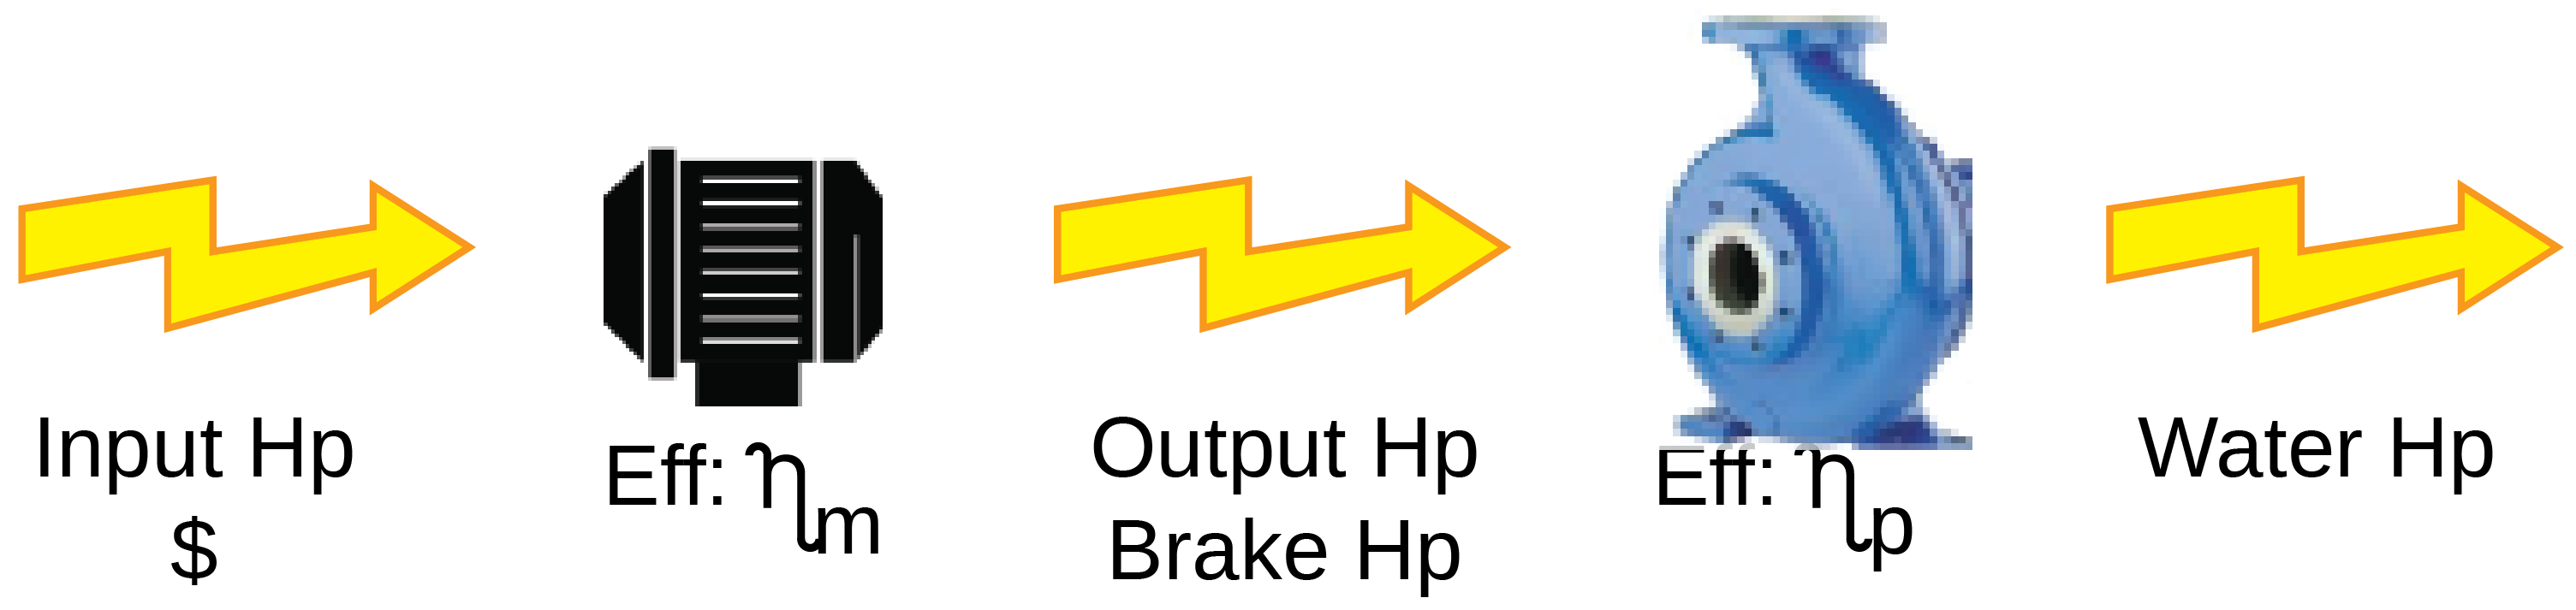
\includegraphics[scale=0.08]{PumpProblem}\\
\vspace{0.4cm}
 $\eta_p=\dfrac{10 \mathrm{WHp}}{15.4 \mathrm{BHp}} \times 100=64.94$ or $\boxed{65 \%}$


 
\item The efficiency of a well pump is determined to be $75 \%$. The efficiency of the motor is estimated at $94 \%$. What is the efficiency of the well?

 \vspace{0.2cm}
$Well \enspace efficiency=\eta_m * \eta_p \implies 0.94 \times 0.75=0.705 \times 100=70.5 \%$
 \vspace{0.2cm}

\vspace{0.32cm}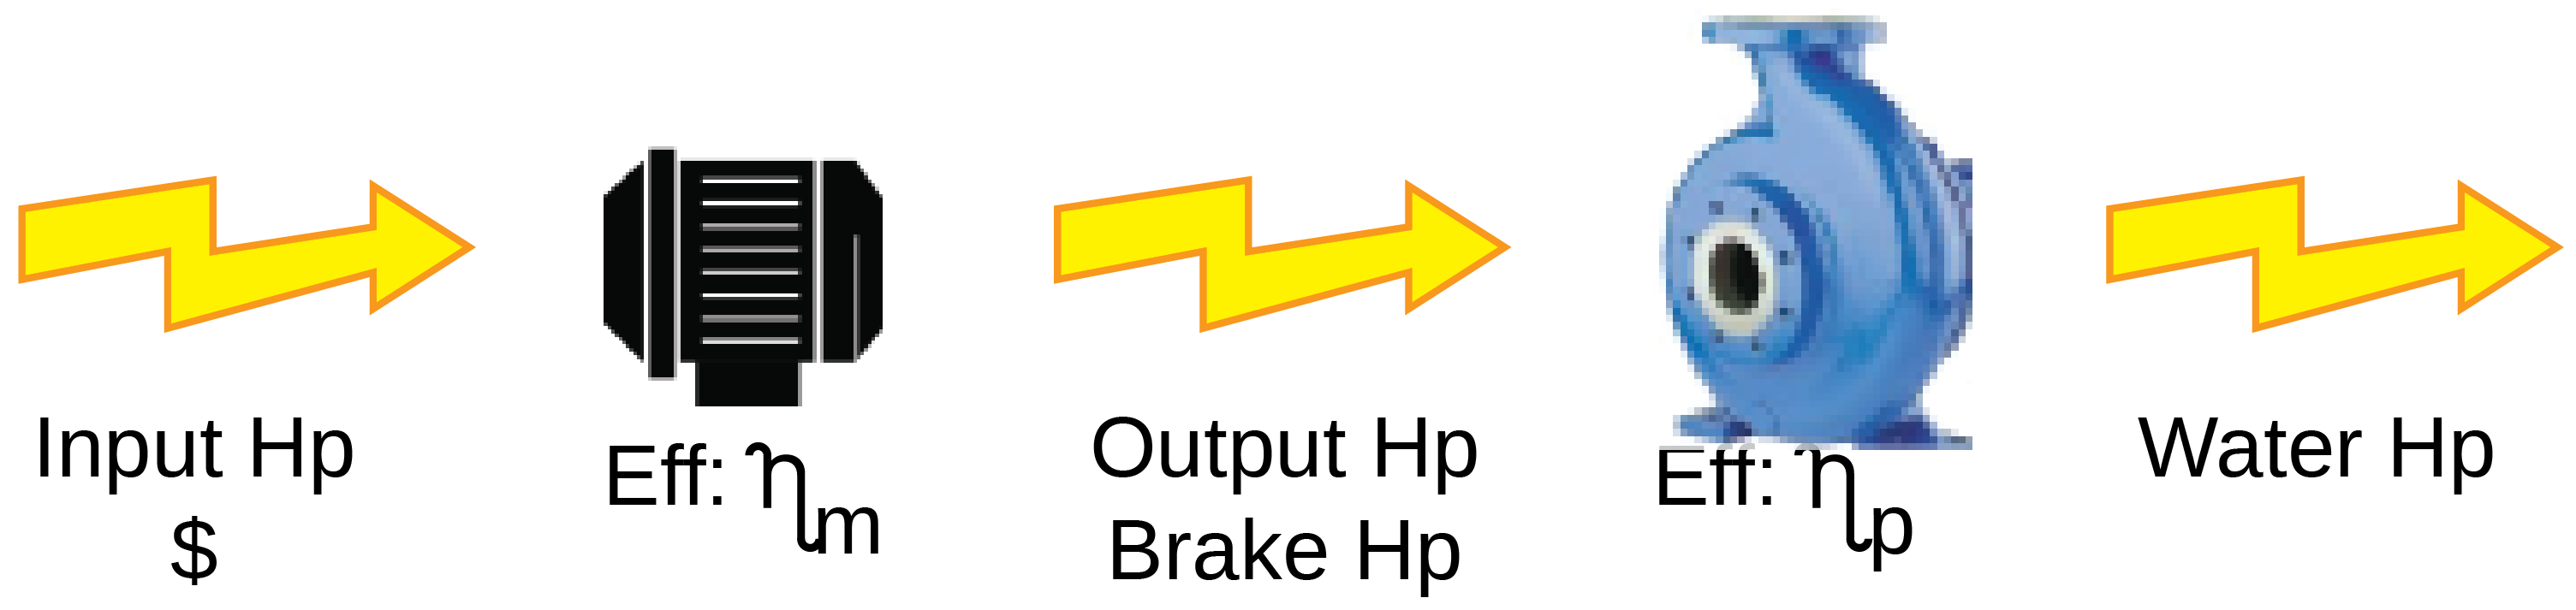
\includegraphics[scale=0.08]{PumpProblem}\\
 \vspace{0.2cm}
$\eta_p=\dfrac{25 \mathrm{\enspace Water \enspace Hp}}{48 \mathrm{\enspace brake \enspace Hp}} \times 100=52 \%$
  \vspace{0.4cm}
  
  
\item If a motor is $85 \%$ efficient and the output of the motor is determined to be 10
$\mathrm{BHp}$, what is the electrical horsepower requirement of the motor?


  \vspace{0.2cm}
 \vspace{0.4cm}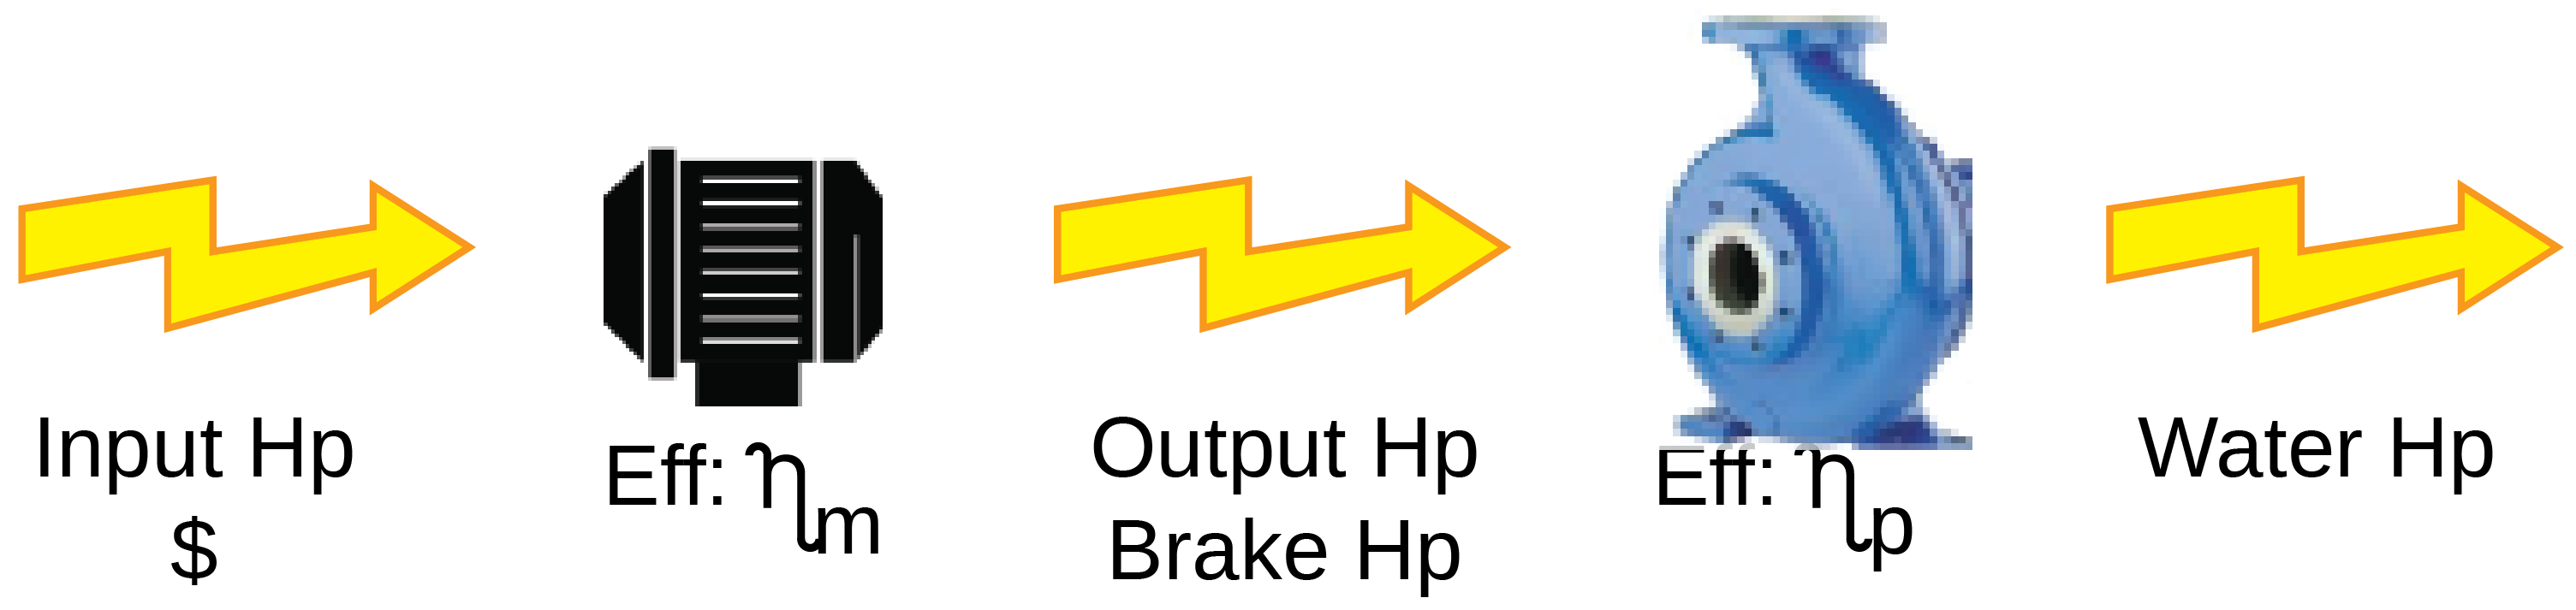
\includegraphics[scale=0.08]{PumpProblem}\\
 \vspace{0.2cm}
 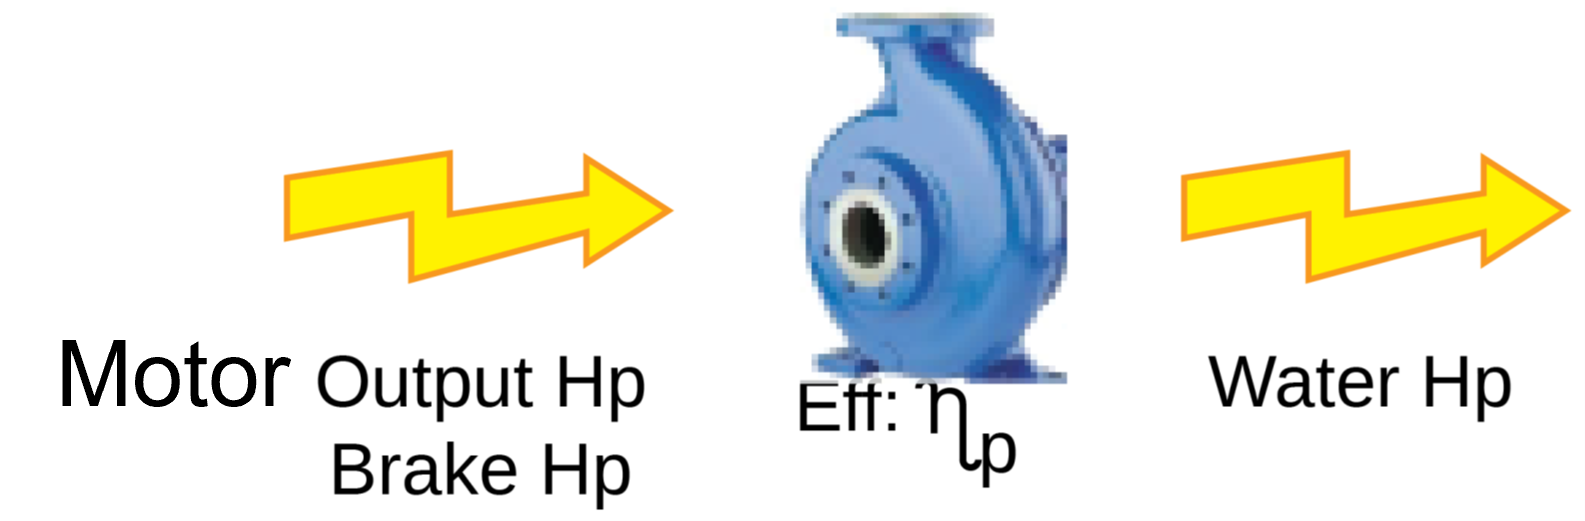
\includegraphics[scale=0.32]{PumpingProblemPump}\\
 \vspace{0.2cm}
$\dfrac{10 \mathrm{BHp}}{0.85}=11.8 \mathrm{EHp \enspace or \enspace Input \enspace Hp}$
 \vspace{0.4cm}
 

\item The water horsepower of a well with a submersible pump has been calculated at 8.2 WHp. The Output of the electric motor is measured as $10.3 \mathrm{BHp}$. What is the efficiency of the pump?


 
  \vspace{0.2cm}
 \vspace{0.08cm}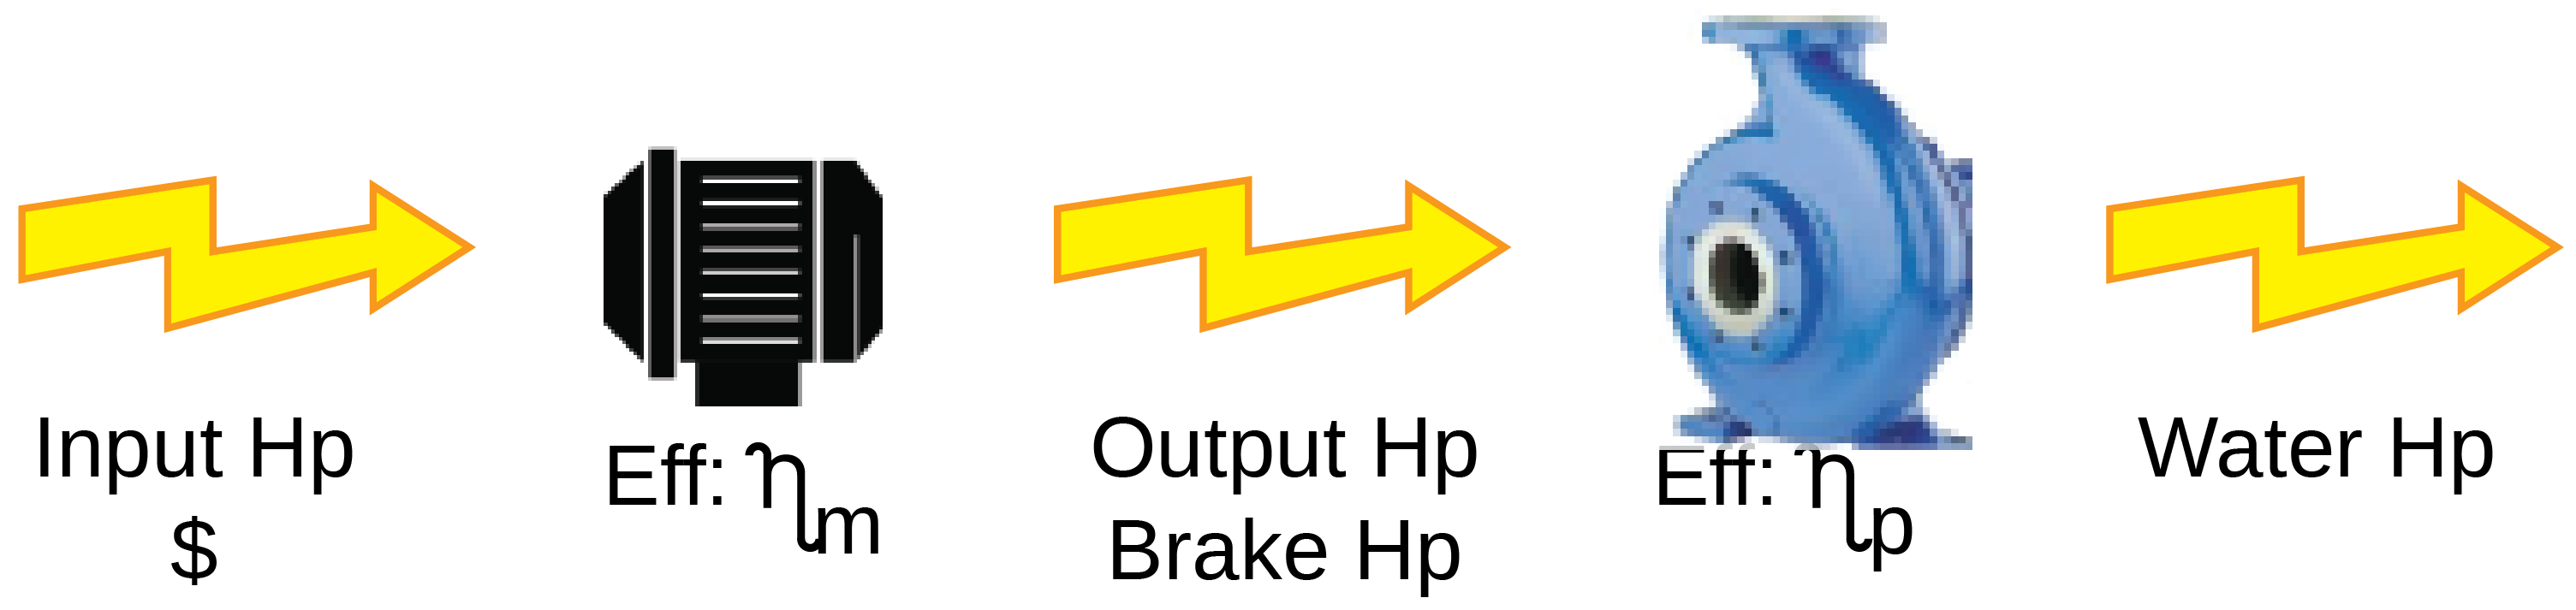
\includegraphics[scale=0.08]{PumpProblem}\\
 \vspace{0.2cm}
 \includegraphics[scale=0.32]{PumpingProblempump}\\
 \vspace{0.2cm}
$\eta_p=\dfrac{82 \mathrm{\enspace W \enspace Hp}}{10.3 \mathrm{\enspace BHp}} \times 100=79.6 \%$
 \vspace{0.2cm}
 
 
 
 
   \item If a pump is operating at 2,200 gpm and 60 feet of head, what is the water
horsepower? If the pump efficiency is 71\%, what is the brake horsepower?\\
\vspace{0.4cm}
water Hp = flow * head\\
$2,200GPM*60ft*\dfrac{Hp}{3,960 GPM-ft}=\boxed{Water \enspace Hp = 33.3Hp}$\\
\vspace{0.4cm}
pump Hp = brake Hp * pump efficiency\\
$brake \enspace Hp = \dfrac{33.3}{0.71}=\boxed{Brake \enspace Hp=47Hp}$
 \vspace{0.2cm}

\item The water horsepower of a pump is $10 \mathrm{Hp}$ and the brake horsepower output of the motor is $15.4 \mathrm{Hp}$. What is the efficiency of the pump?\\
 \vspace{0.2cm}
 \vspace{0.4cm}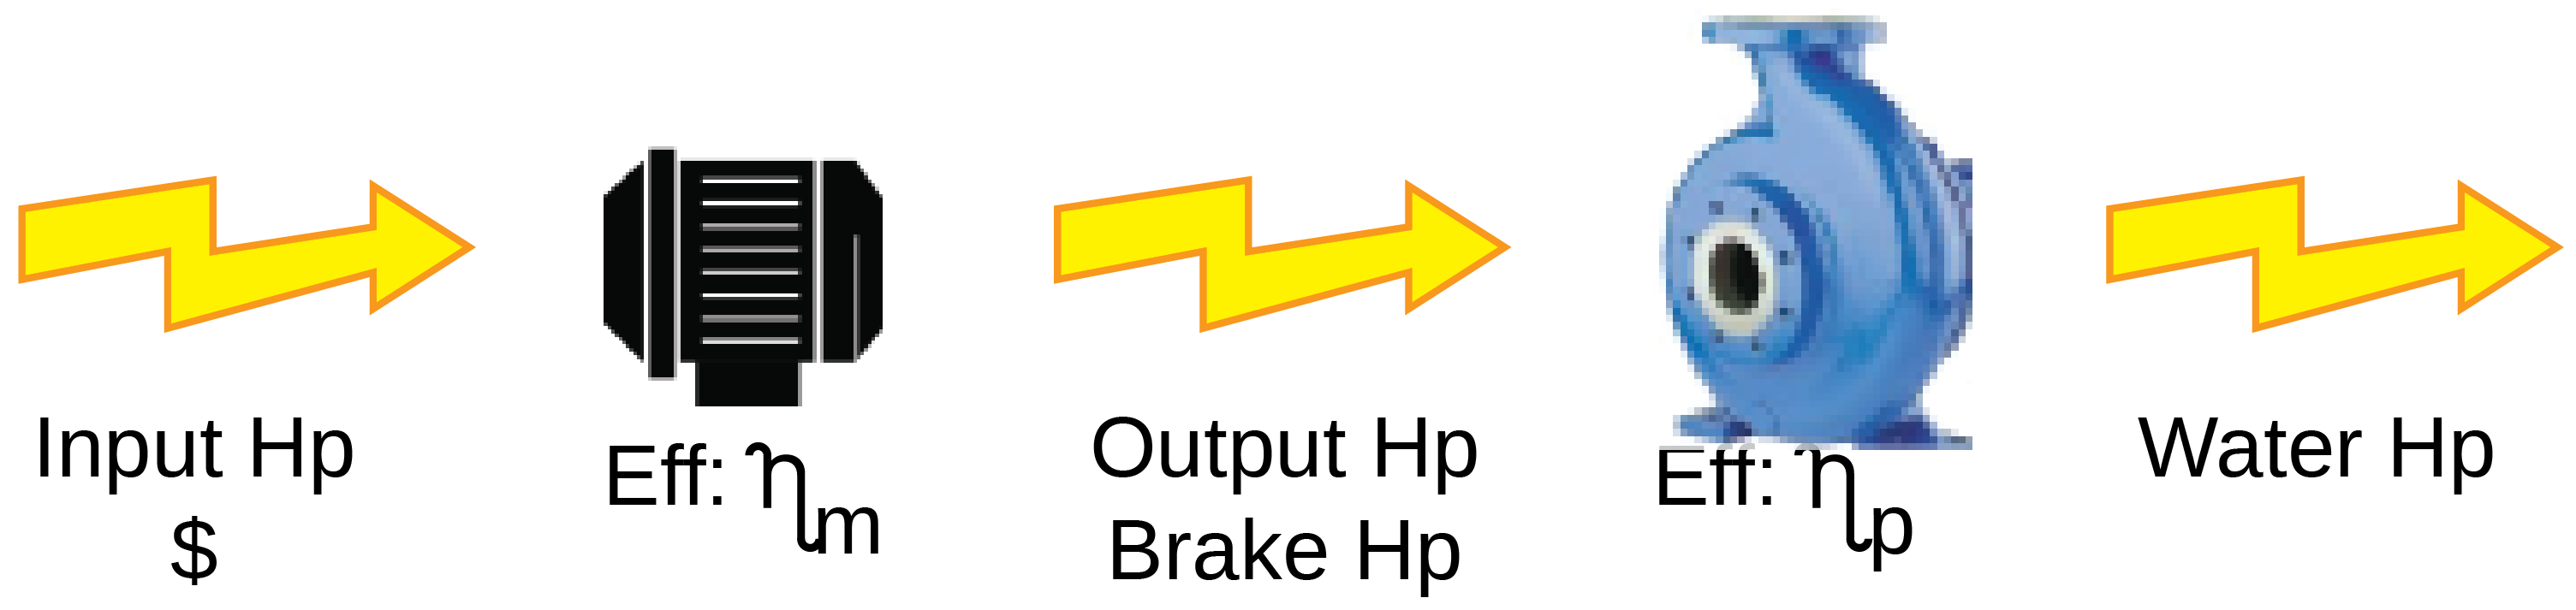
\includegraphics[scale=0.08]{PumpProblem}\\
 \vspace{0.2cm}
 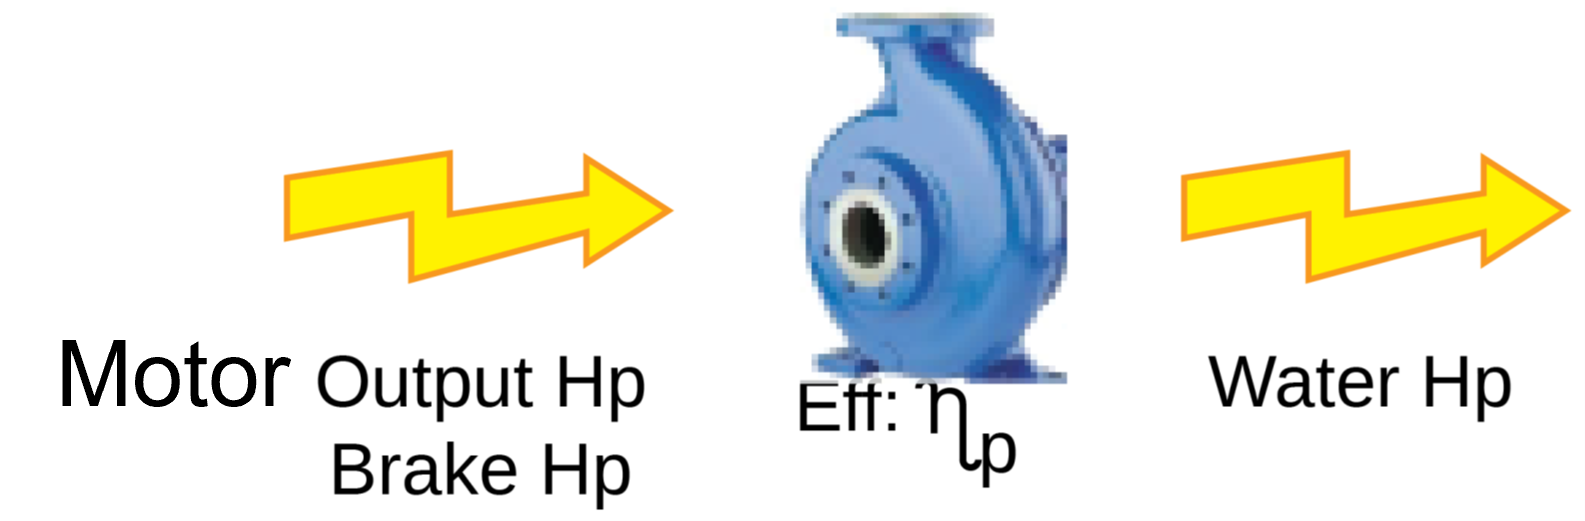
\includegraphics[scale=0.32]{PumpingProblemPump}
 $\eta_p=\dfrac{10 \mathrm{WHp}}{15.4 \mathrm{BHp}} \times 100=\boxed{65 \%}$
 \vspace{0.2cm}

\item The water horsepower of a pump is $25 \mathrm{Hp}$ and the brake horsepower output of the motor is $48 \mathrm{Hp}$. What is the efficiency of the pump?\\
  \vspace{0.2cm}
 \vspace{0.32cm}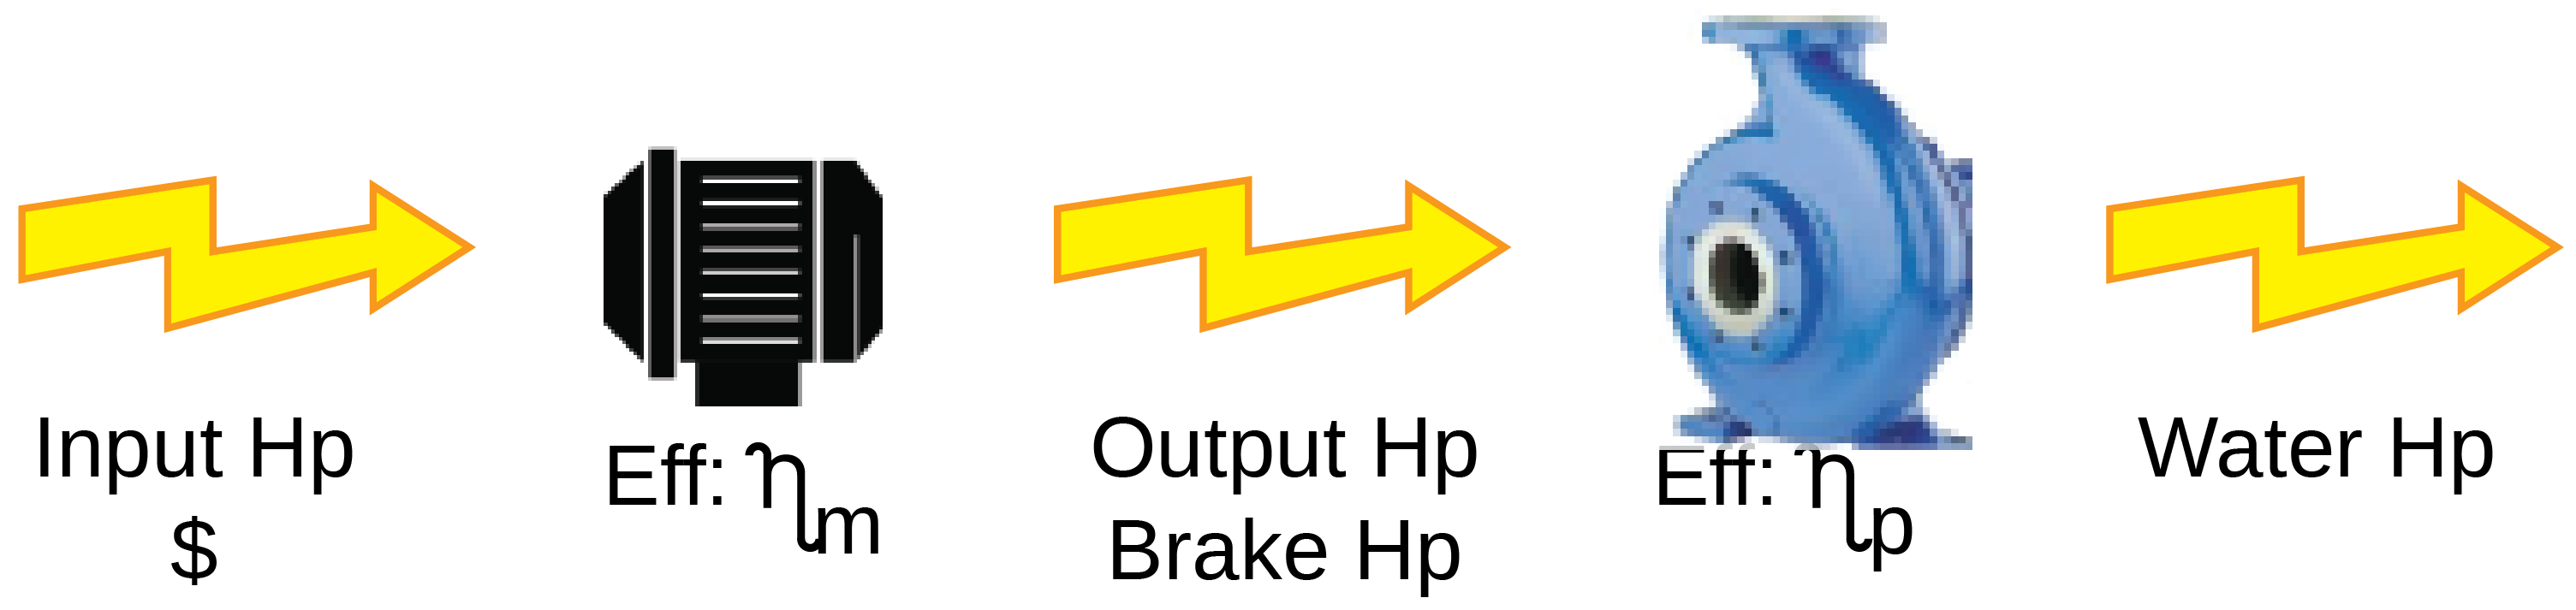
\includegraphics[scale=0.08]{PumpProblem}\\
 \vspace{0.2cm}
 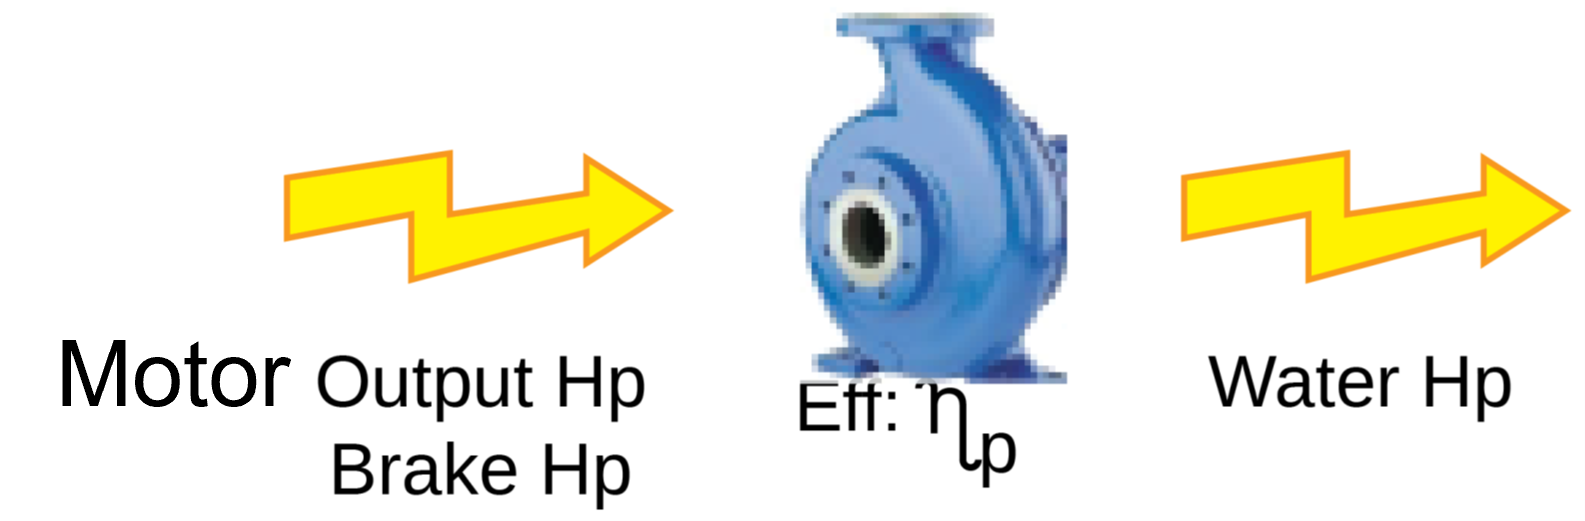
\includegraphics[scale=0.4]{PumpingProblemPump}\\
 \vspace{0.2cm}
$\eta_p=\dfrac{25 \mathrm{\enspace Water \enspace Hp}}{48 \mathrm{\enspace brake \enspace Hp}} \times 100=\boxed{52 \%}$
  \vspace{0.4cm}


\item The efficiency of a well pump is determined to be $75 \%$. The efficiency of the motor is estimated at $94 \%$. What is the efficiency of the well?\\

 \vspace{0.2cm}
$Well \enspace efficiency=\eta_m * \eta_p \implies 0.94 \times 0.75=0.705 \times 100=\boxed{71 \%}$
 \vspace{0.2cm}

\item If a motor is $85 \%$ efficient and the output of the motor is determined to be 10
$\mathrm{BHp}$, what is the electrical horsepower requirement of the motor?

 \vspace{0.4cm}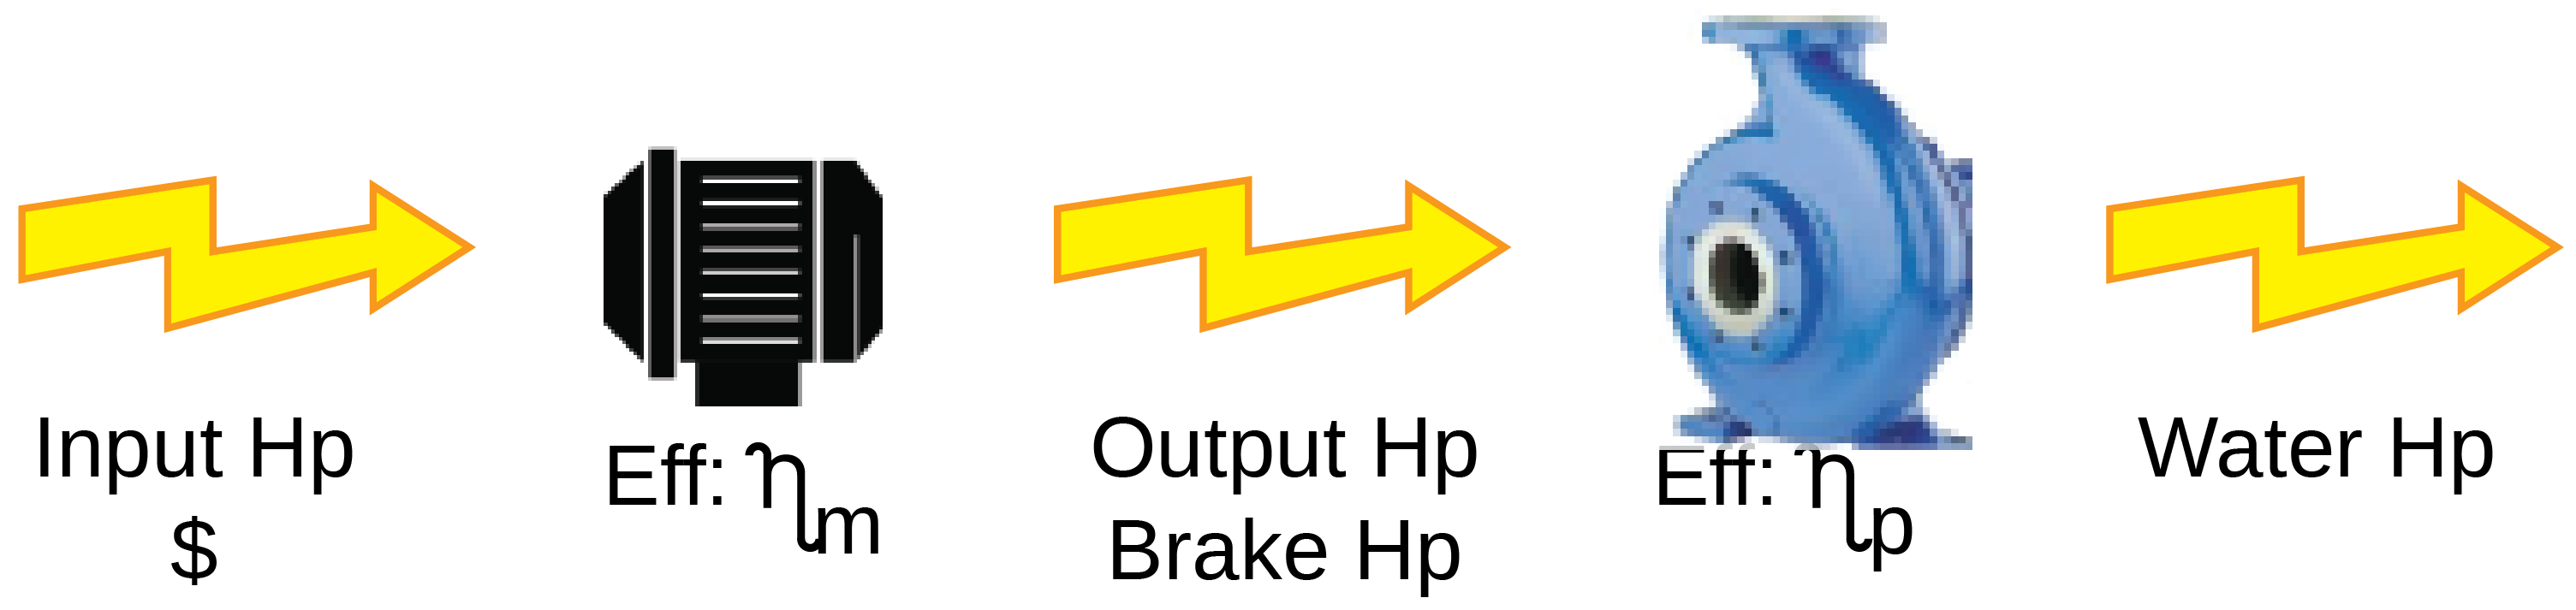
\includegraphics[scale=0.08]{PumpProblem}\\
 \vspace{0.2cm}
 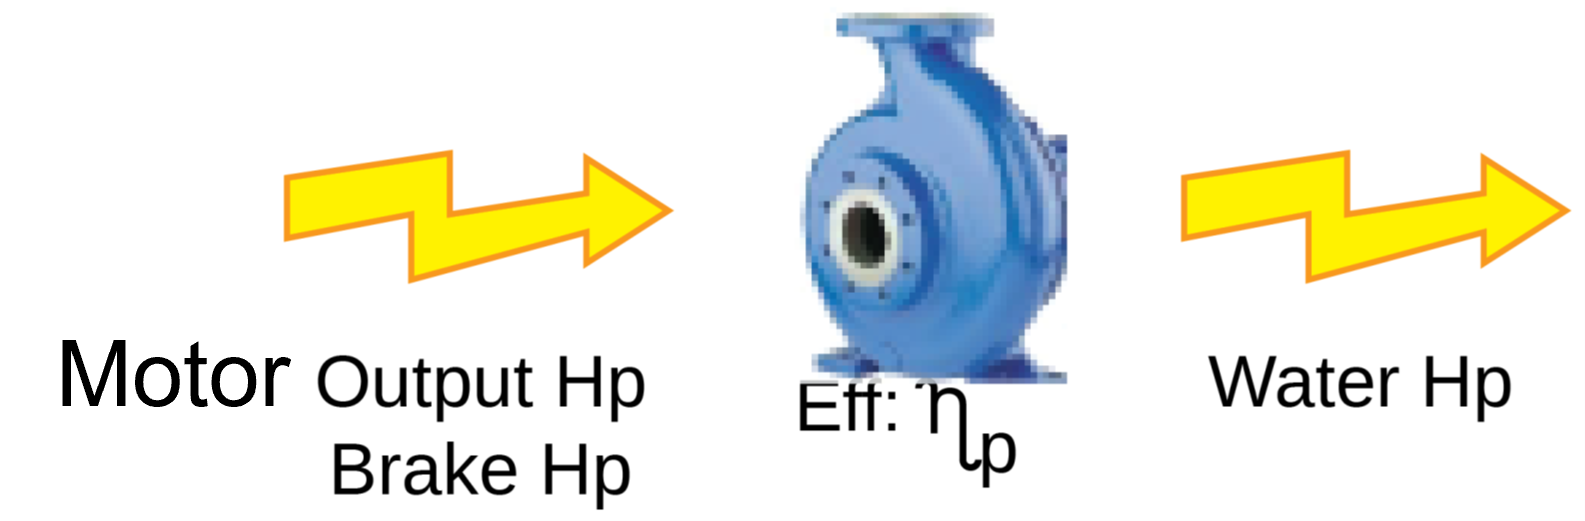
\includegraphics[scale=0.32]{PumpingProblemPump}\\
 \vspace{0.2cm}
$\dfrac{10 \mathrm{BHp}}{0.85}=\boxed{12 \mathrm{EHp \enspace or \enspace Input \enspace Hp}}$
 \vspace{0.4cm}



  \item Water is being pumped from a reservoir to a storage tank on a hill. The elevation difference between water levels is 1200 feet. Find the pump size required to fill the tank at a rate of 120 gpm. Express your answer in horsepower.
  
  \vspace{0.4cm}
water Hp = flow * head\\
\vspace{0.4cm}
$\mathrm{Water} \enspace \mathrm{Hp} = 120 \enspace \mathrm{gpm}*1,200 \enspace ft*\dfrac{\mathrm{Hp}}{3,960 \enspace \mathrm{gpm-ft}}=\boxed{ 37 \enspace \mathrm{Hp}}$\\
\vspace{0.2cm}


  \item A $25 \mathrm{hp}$ pump is used to dewater a lake. If the pump runs for 8 hours a day for 7 days a week, how much will it cost to run the pump for one week? Assume energy costs $\$ 0.07$ per kilowatt hour.
  
  \vspace{0.4cm}
$25 \enspace \mathrm{Hp}\dfrac{0.746 \enspace \mathrm{kW}}{\mathrm{Hp}}*\dfrac{8 \enspace \mathrm{hrs}}{\mathrm{day}}*\dfrac{7 \enspace \mathrm{days}}{\mathrm{month}}*\dfrac{\$0.07}{\mathrm{kWh}}=\boxed{\dfrac{\$73.1}{\mathrm{week}}}$\\
\vspace{0.2cm}

\newpage

  \item A pump station is used to lift water 50 feet above the pump station to a storage tank. The pump rate is $500 \mathrm{gpm}$. If the pump has an efficiency of $85 \%$ and the motor has an efficiency of $90 \%$, find each of the following: Water Horsepower, Brake Horsepower, Motor Horsepower, and Wire-to-Water Efficiency.\\

\tikzstyle{block} = [rectangle, draw, fill=red!40, 
    text width=3.5em, text centered, rounded corners, minimum height=1.5em]
\tikzstyle{arrow} = [draw, -latex']
\begin{figure}[h!]
\centering
\begin{tikzpicture}[node distance =1.5cm, auto]
    % Place nodes
    \draw ++(-3.6,-1.5) node [block] (Process) {\tiny{\textbf{Step 3:}\\}};
    \draw ++(-2,-1.5) node [block] (Process) {\tiny{$\eta_m=90\%$}};
    \draw ++(-0.4,-1.5) node [block] (Process) {\tiny{Step 2}};
    \draw ++(1.2,-1.5) node [block] (Process) {\tiny{$\eta_p=85\%$}};
    \draw ++(2.8,-1.5) node [block] (Process) {\tiny{Step 1}};

    \node[inner sep=0pt] (pump) at (-0.4,0)
    {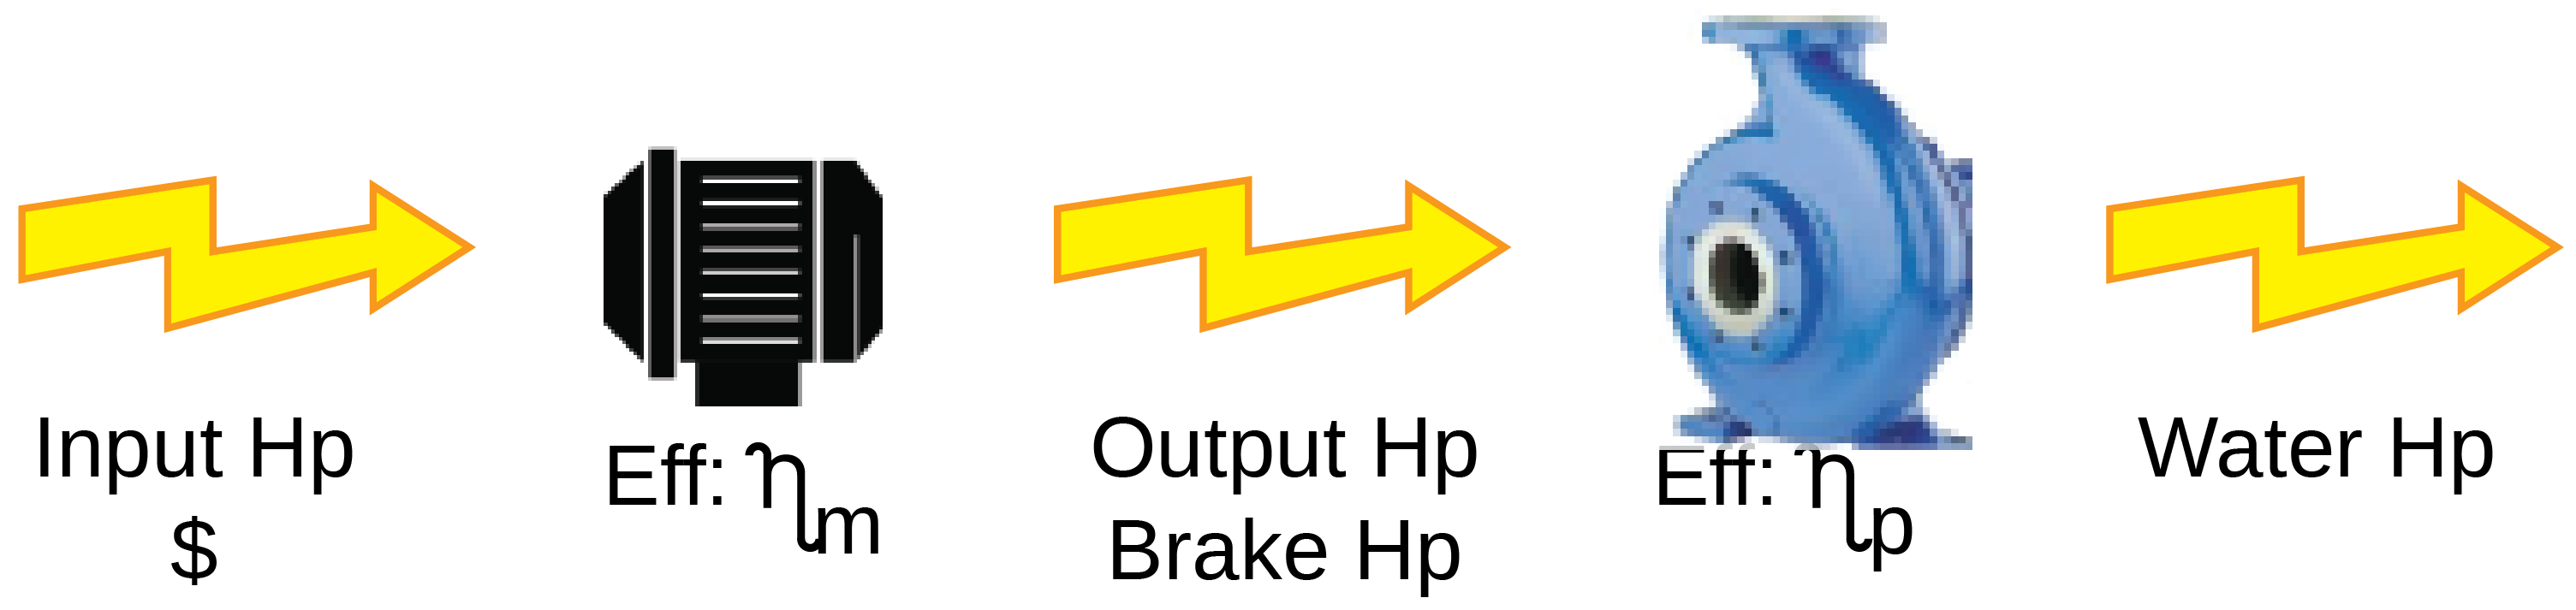
\includegraphics[width=.75\textwidth]{PumpProblem}};

\end{tikzpicture}

\end{figure}
\textbf{Step 1:}\\
water Hp = flow * head\\
$\mathrm{water} \enspace \mathrm{Hp} = 500 \enspace \mathrm{gpm}*50 \enspace ft*\dfrac{\mathrm{Hp}}{3,960 \enspace \mathrm{gpm-ft}}$\\
$=\boxed{ 6.3 \enspace \mathrm{WHp}}$\\ 
\vspace{0.1cm}
  \textbf{Step 2:}\\
$\mathrm{pump \enspace efficiency} =\dfrac{\mathrm{water \enspace Hp}}{\mathrm{brake \enspace Hp}}$\\
$ \implies \mathrm{brake \enspace Hp}=\dfrac{\mathrm{water \enspace Hp}}{\mathrm{pump \enspace efficiency}} = \dfrac{6.3}{0.85}=\boxed{7.4 \enspace \mathrm{Hp}}$\\
\vspace{0.1cm}
  \textbf{Step 3:}\\
$\mathrm{motor \enspace efficiency} =\dfrac{\mathrm{brake \enspace Hp}}{\mathrm{input \enspace Hp}}$\\
$ \implies \mathrm{input \enspace \enspace Hp}=\dfrac{\mathrm{brake \enspace Hp}}{\mathrm{motor \enspace efficiency}}= \dfrac{7.4}{0.9}=\boxed{8.2 \enspace \mathrm{Hp}}$\\
\vspace{0.1cm}
  \textbf{Step 4:}\\

$\mathrm{Wire-to-water} \enspace \mathrm{efficiency}=\eta_m * \eta_p * 100$\\
$\implies 0.9 \times 0.85 \times 100=\boxed{77 \%}$

\newpage

  \item Find the brake horsepower for a pump given the following information:\\
   Total Dynamic Head $=75$ feet,\\
   Pump Rate $=150$ gpm\\
   Pump Efficiency $=90 \%$\\
   Motor Efficiency $=85 \%$\\
  \vspace{0.4cm}
water Hp = flow * head\\
$150 \enspace \mathrm{GPM}*75\mathrm{ft}*\dfrac{Hp}{3,960 GPM-ft}=\boxed{Water \enspace Hp = 2.8Hp}$\\
\vspace{0.4cm}
pump Hp = brake Hp * pump efficiency\\
$brake \enspace Hp = \dfrac{2.8}{0.9}=\boxed{Brake \enspace Hp=3.1Hp}$
 \vspace{0.2cm}
 
 
 


  \item If a pump is operating at 2,200 gpm and 60 feet of head, what is the water
horsepower? If the pump efficiency is 71\%, what is the brake horsepower?\\
  \vspace{0.2cm}
Solution:\\
\vspace{0.4cm}
water Hp = flow * head\\
$2,200GPM*60ft*\dfrac{Hp}{3,960 GPM-ft}=\boxed{Water \enspace Hp = 33.3Hp}$\\
\vspace{0.4cm}
pump Hp = brake Hp * pump efficiency\\
$brake \enspace Hp = \dfrac{33.3}{0.71}=\boxed{Brake \enspace Hp=47Hp}$
 \vspace{0.2cm}

\item The water horsepower of a pump is $10 \mathrm{Hp}$ and the brake horsepower output of the motor is $15.4 \mathrm{Hp}$. What is the efficiency of the pump?\\
  \vspace{0.2cm}
Solution:\\ 
 \vspace{0.2cm}
 \vspace{0.4cm}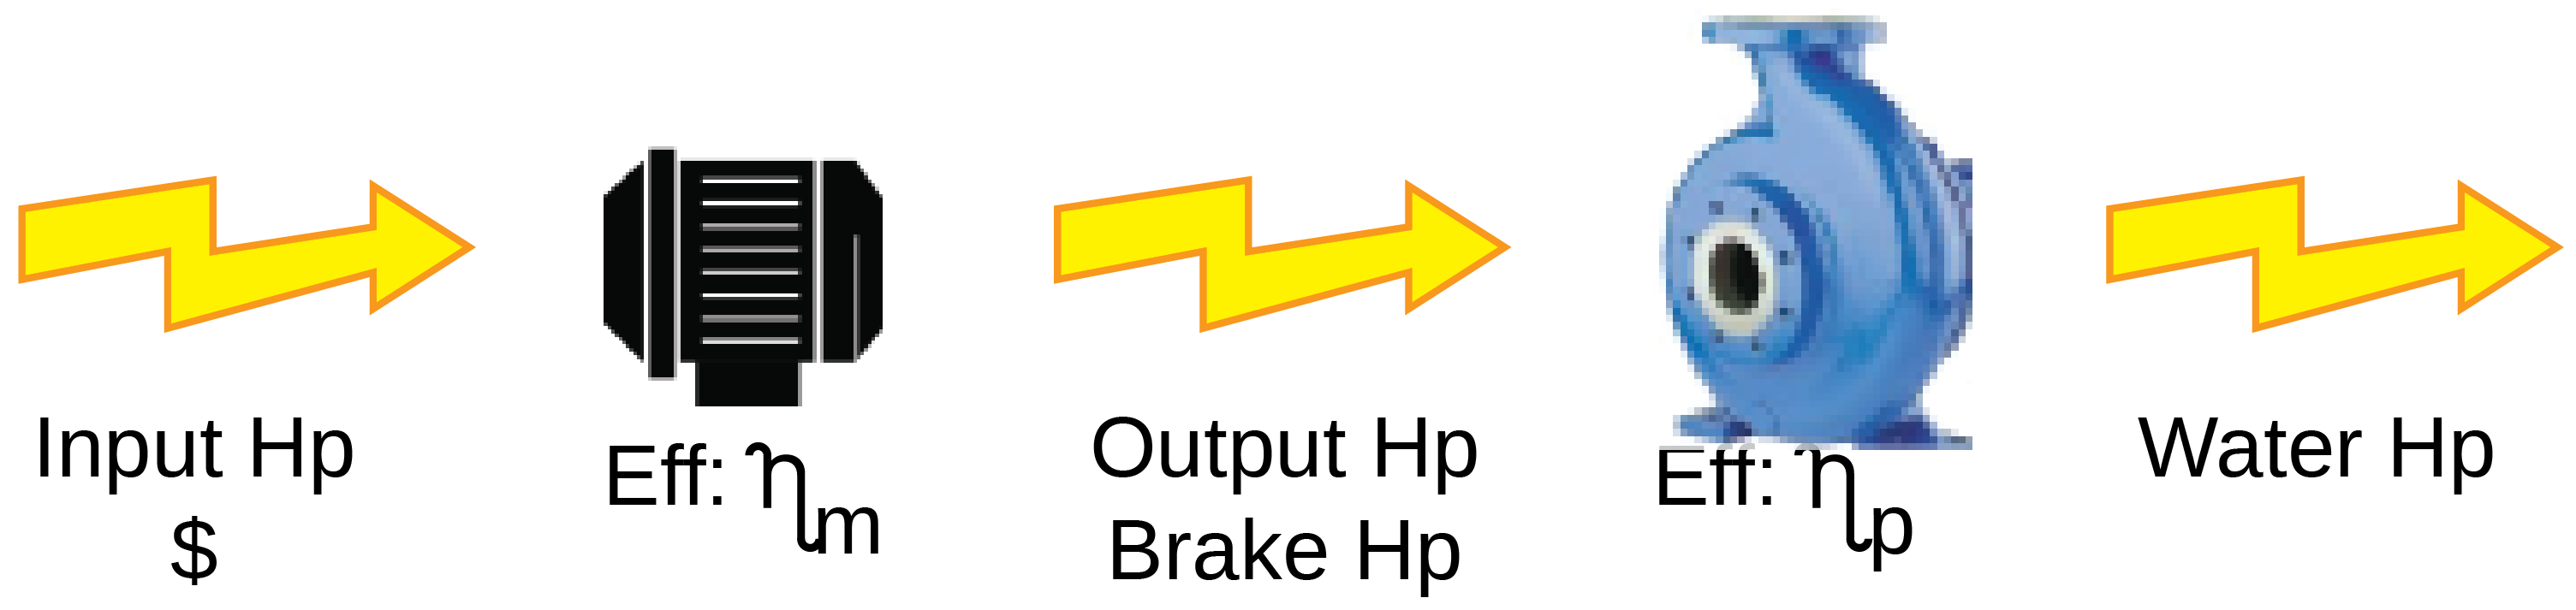
\includegraphics[scale=0.08]{PumpProblem}\\
 \vspace{0.2cm}
 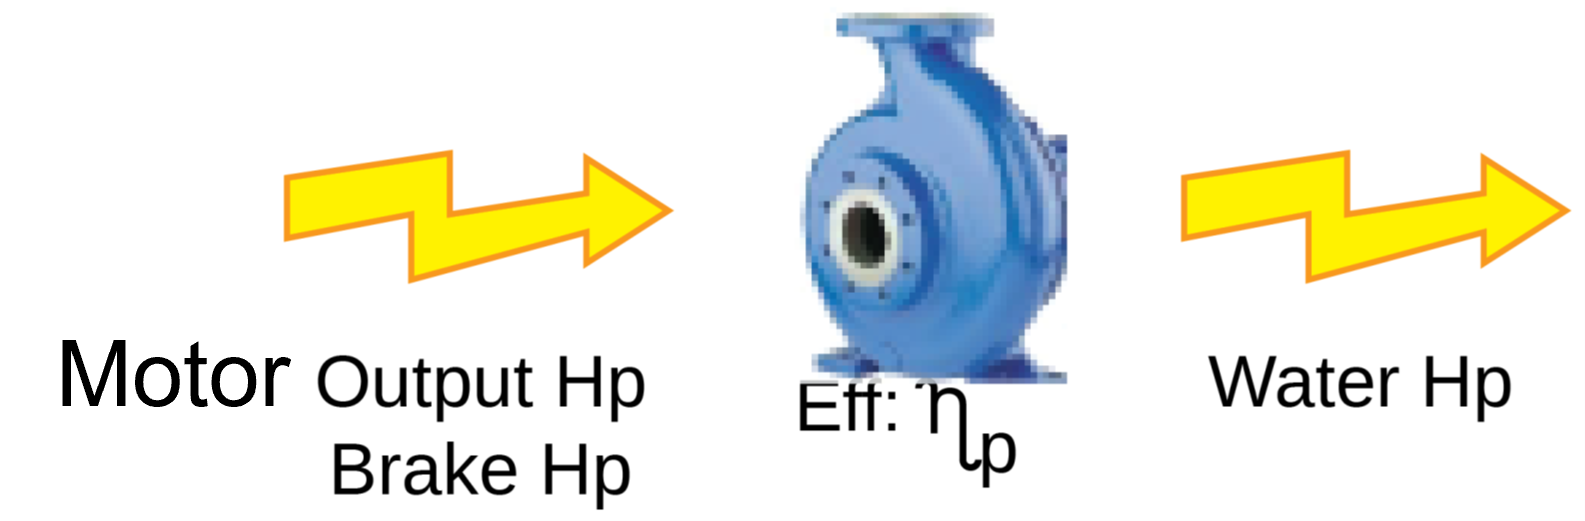
\includegraphics[scale=0.32]{PumpingProblemPump}
 $\eta_p=\dfrac{10 \mathrm{BHp}}{15.4 \mathrm{EHp}} \times 100=\boxed{65 \%}$
 \vspace{0.2cm}

\item The water horsepower of a pump is $25 \mathrm{Hp}$ and the brake horsepower output of the motor is $48 \mathrm{Hp}$. What is the efficiency of the pump?\\
  \vspace{0.2cm}
Solution:\\
  \vspace{0.2cm}
 \vspace{0.32cm}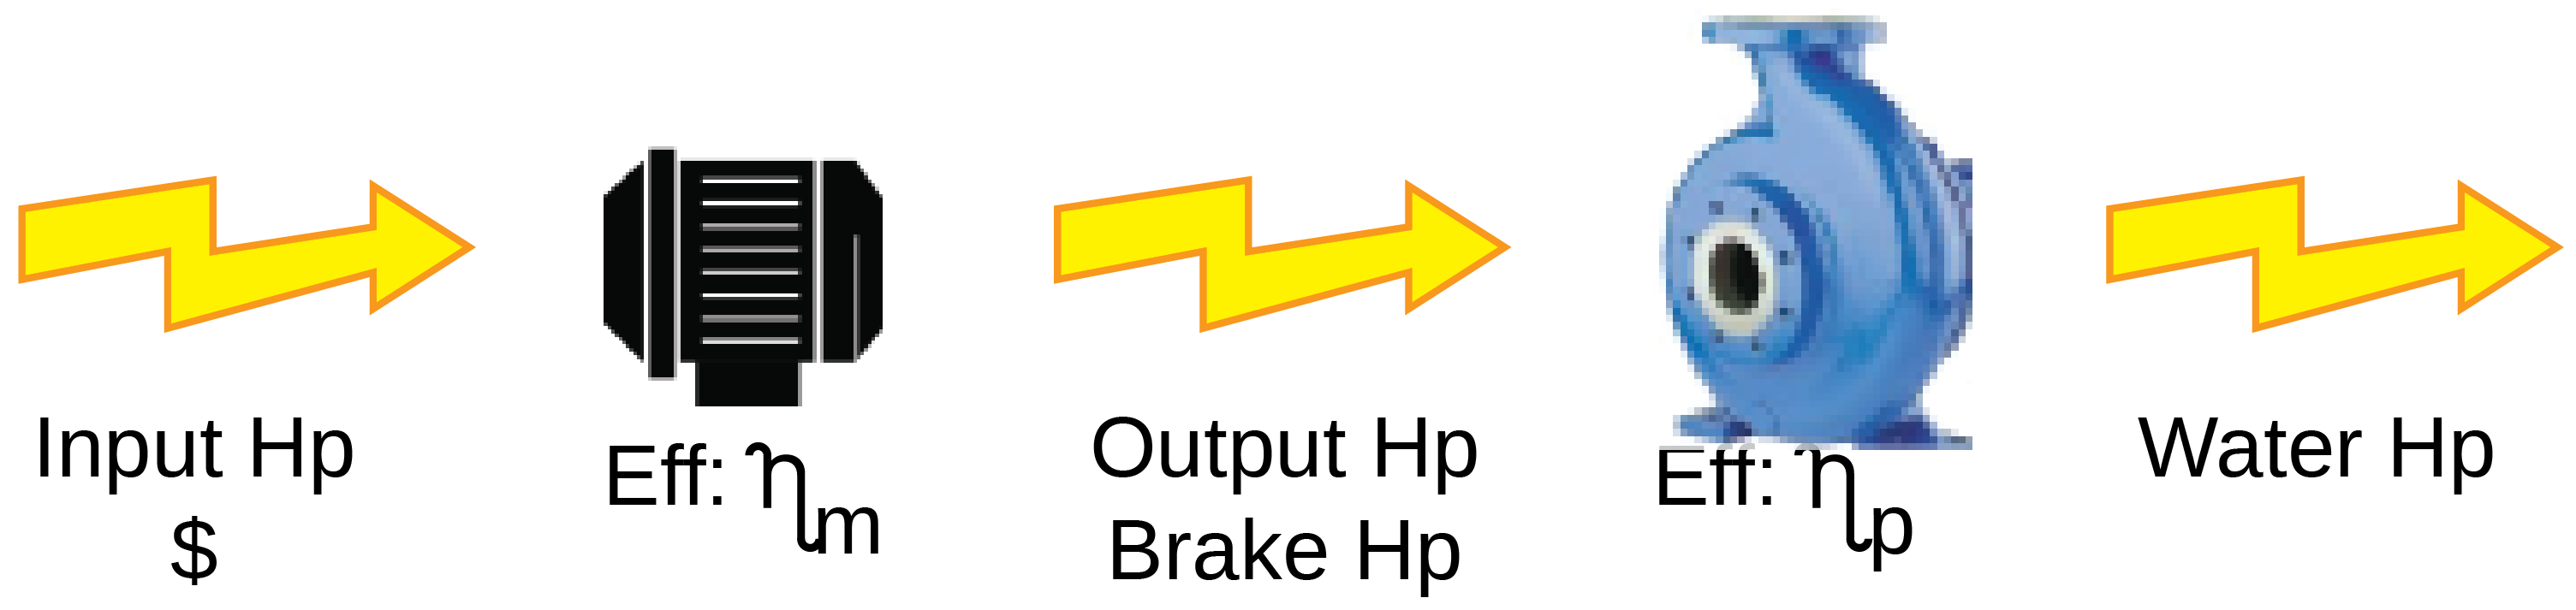
\includegraphics[scale=0.08]{PumpProblem}\\
 \vspace{0.2cm}
 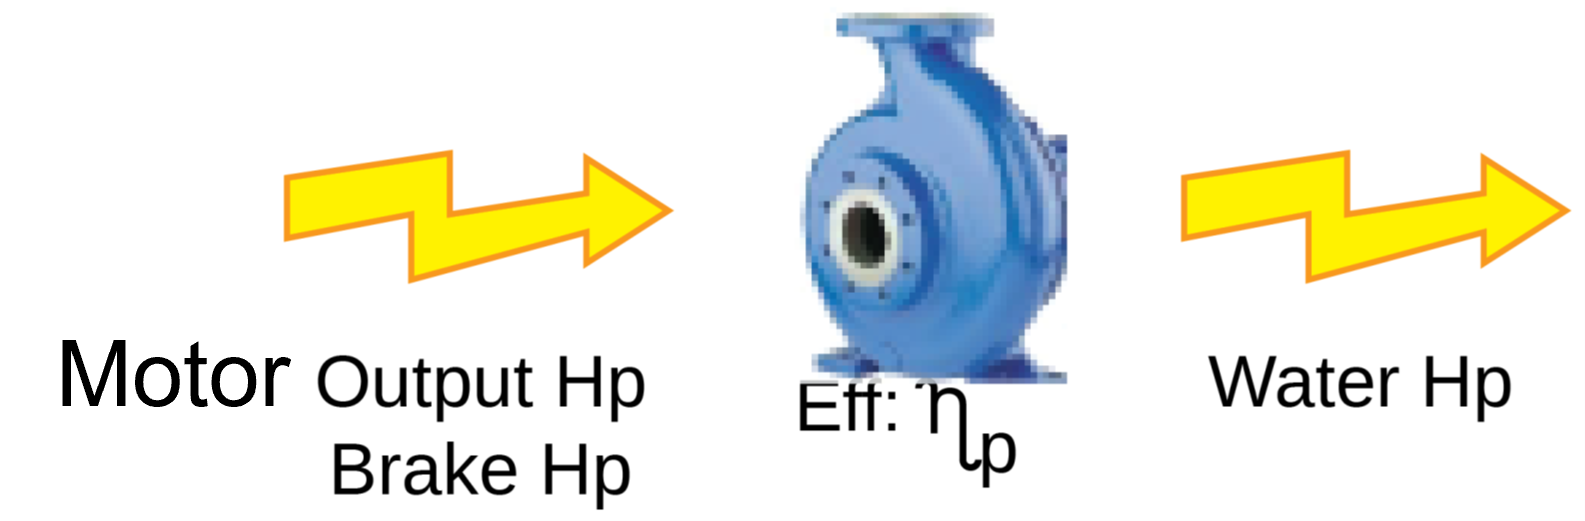
\includegraphics[scale=0.4]{PumpingProblemPump}
 \vspace{0.2cm}
$\eta_p=\dfrac{25 \mathrm{\enspace Water \enspace Hp}}{48 \mathrm{\enspace brake \enspace Hp}} \times 100=\boxed{52 \%}$
  \vspace{0.4cm}
 \item Solution:\\ 
 \vspace{0.2cm}
$Well \enspace efficiency=\eta_m * \eta_p \implies 0.94 \times 0.75=0.705 \times 100=\boxed{71 \%}$
 \vspace{0.2cm}

\item The efficiency of a well pump is determined to be $75 \%$. The efficiency of the motor is estimated at $94 \%$. What is the efficiency of the well?\\
Solution:\\
\vspace{0.4cm}
$25 \enspace \mathrm{Hp}\dfrac{0.746 \enspace \mathrm{kW}}{\mathrm{Hp}}*\dfrac{8 \enspace \mathrm{hrs}}{\mathrm{day}}*\dfrac{7 \enspace \mathrm{days}}{\mathrm{month}}*\dfrac{\$0.07}{\mathrm{kWh}}=\boxed{\dfrac{\$73.1}{\mathrm{week}}}$\\
\vspace{0.2cm}

\item If a motor is $85 \%$ efficient and the output of the motor is determined to be 10
$\mathrm{BHp}$, what is the electrical horsepower requirement of the motor?\\
  \vspace{0.2cm}
Solution:\\
 \vspace{0.4cm}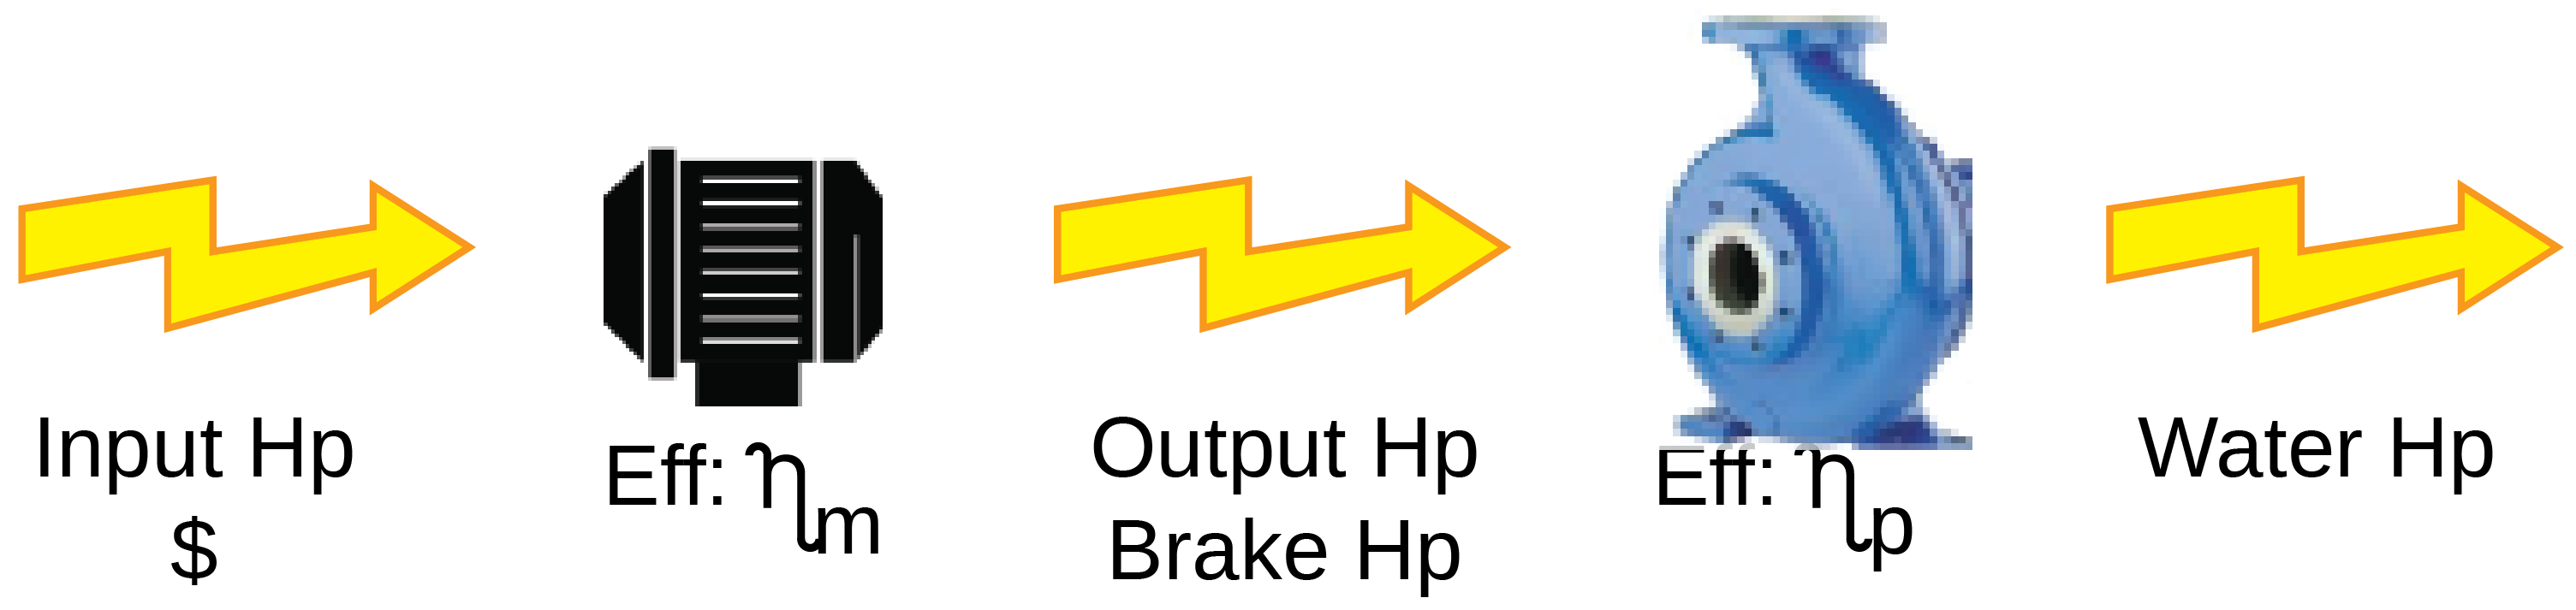
\includegraphics[scale=0.08]{PumpProblem}\\
 \vspace{0.2cm}
 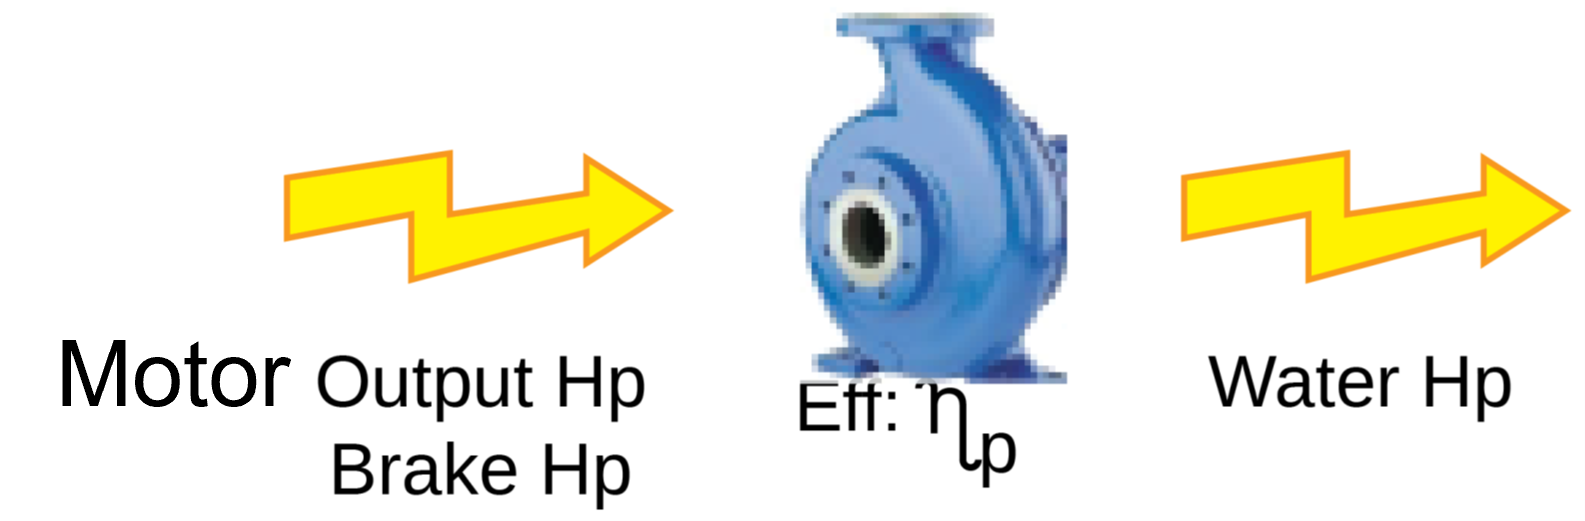
\includegraphics[scale=0.32]{PumpingProblemPump}
 \vspace{0.2cm}
$\dfrac{10 \mathrm{BHp}}{0.85}=\boxed{12 \mathrm{EHp \enspace or \enspace Input \enspace Hp}}$
 \vspace{0.4cm}
 
\item The water horsepower of a well with a submersible pump has been calculated at 8.2 WHp. The Output of the electric motor is measured as $10.3 \mathrm{BHp}$. What is the efficiency of the pump?\\
  \vspace{0.2cm}
Solution:\\ 
  \vspace{0.2cm}
 \vspace{0.08cm}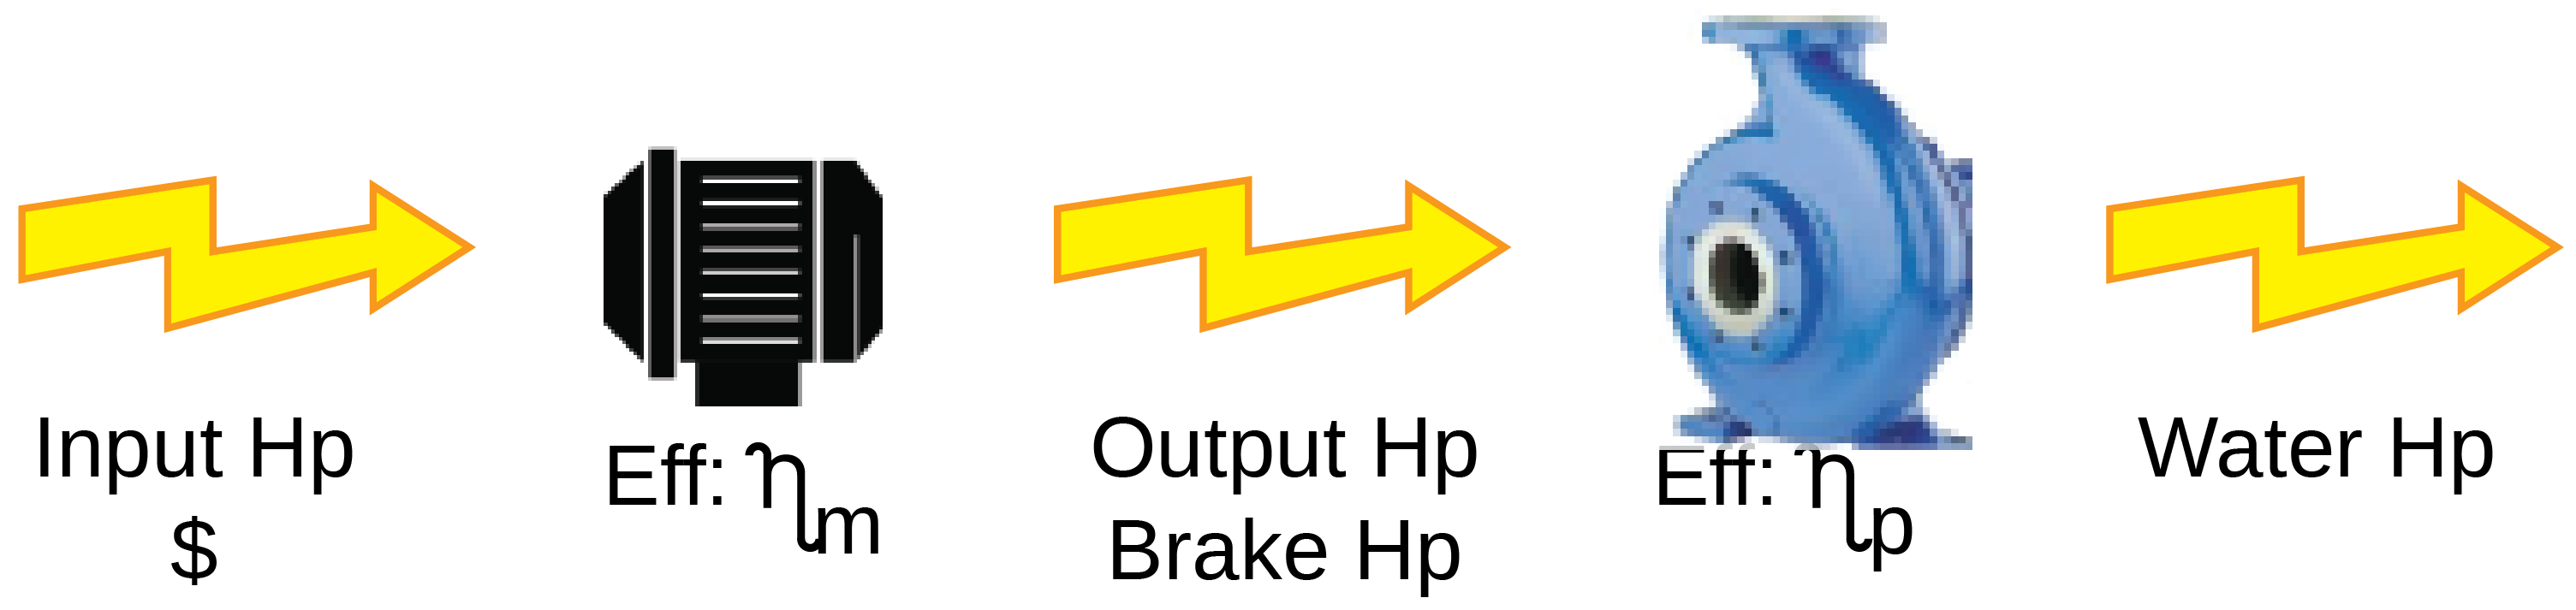
\includegraphics[scale=0.08]{PumpProblem}\\
 \vspace{0.2cm}
 \includegraphics[scale=0.32]{PumpingProblempump}
 \vspace{0.2cm}
$\eta_p=\dfrac{8.2 \mathrm{\enspace W \enspace Hp}}{10.3 \mathrm{\enspace BHp}} \times 100=\boxed{80 \%}$
 \vspace{0.2cm}

  \item Water is being pumped from a reservoir to a storage tank on a hill. The elevation difference between water levels is 1200 feet. Find the pump size required to fill the tank at a rate of 120 gpm. Express your answer in horsepower.\\
  \vspace{0.2cm} 
 Solution:\\
\vspace{0.4cm}
water Hp = flow * head\\
\vspace{0.4cm}
$\mathrm{Water} \enspace \mathrm{Hp} = 120 \enspace \mathrm{gpm}*1,200 \enspace ft*\dfrac{\mathrm{Hp}}{3,960 \enspace \mathrm{gpm-ft}}=\boxed{ 37 \enspace \mathrm{Hp}}$\\
\vspace{0.2cm}

  \item A $25 \mathrm{hp}$ pump is used to dewater a lake. If the pump runs for 8 hours a day for 7 days a week, how much will it cost to run the pump for one week? Assume energy costs $\$ 0.07$ per kilowatt hour.

  \item A pump station is used to lift water 50 feet above the pump station to a storage tank. The pump rate is $500 \mathrm{gpm}$. If the pump has an efficiency of $85 \%$ and the motor has an efficiency of $90 \%$, find each of the following: Water Horsepower, Brake Horsepower, Motor Horsepower, and Wire-to-Water Efficiency.\\
 \vspace{0.2cm}
Solution:\\
 \vspace{0.4cm}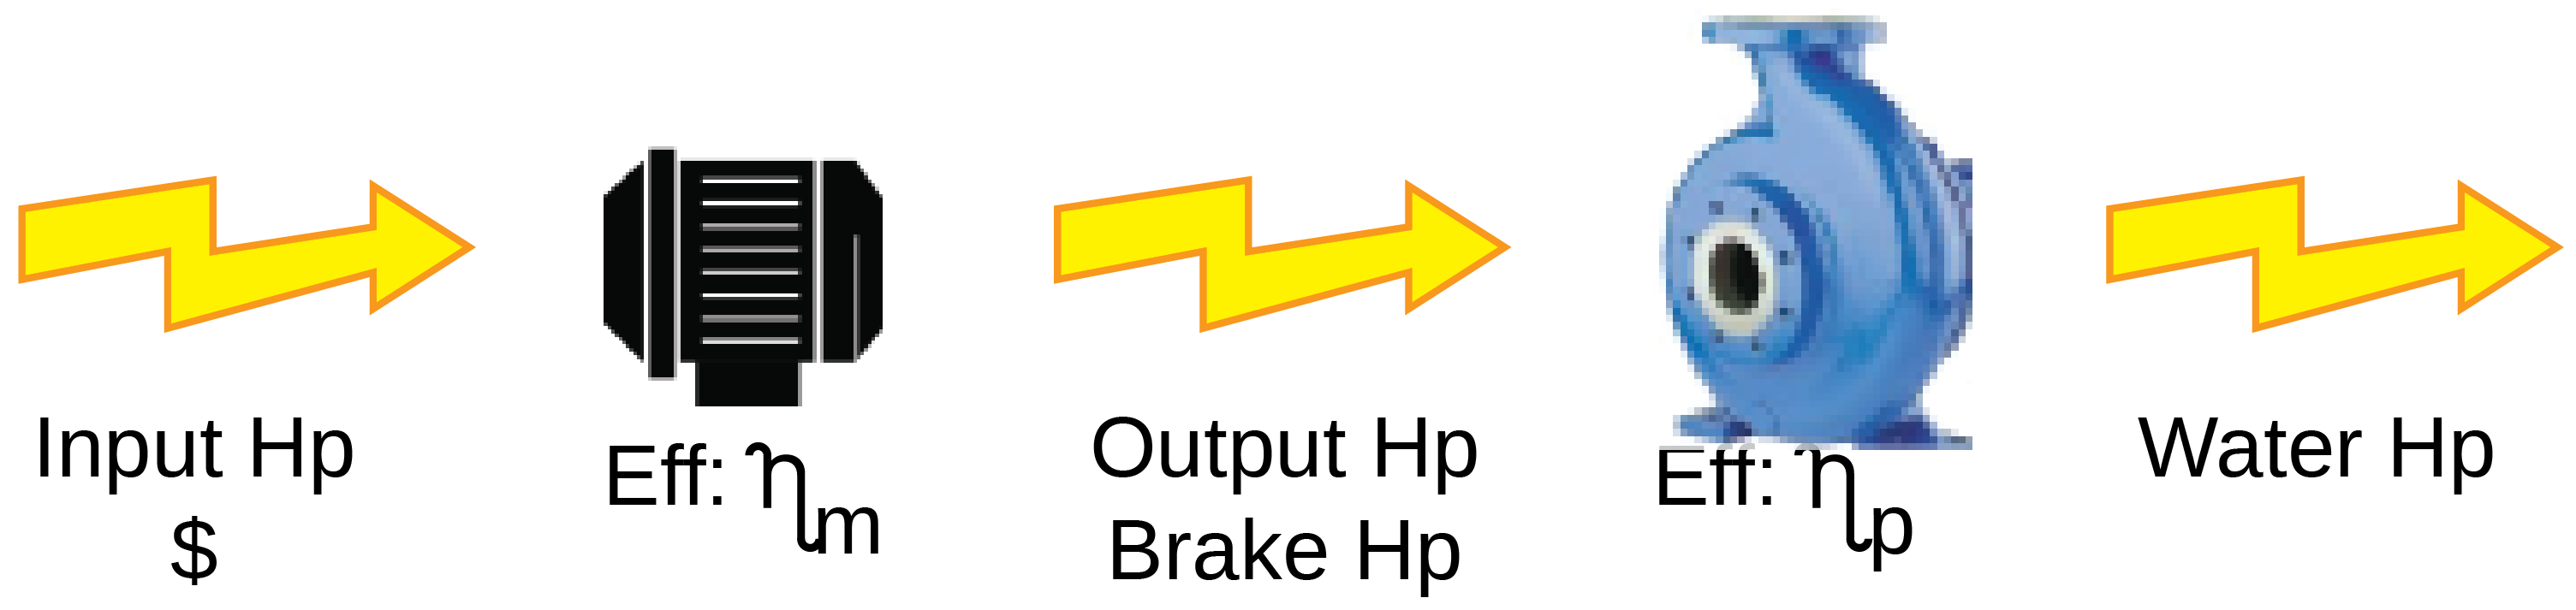
\includegraphics[scale=0.08]{PumpProblem}\\
 \vspace{0.2cm}
 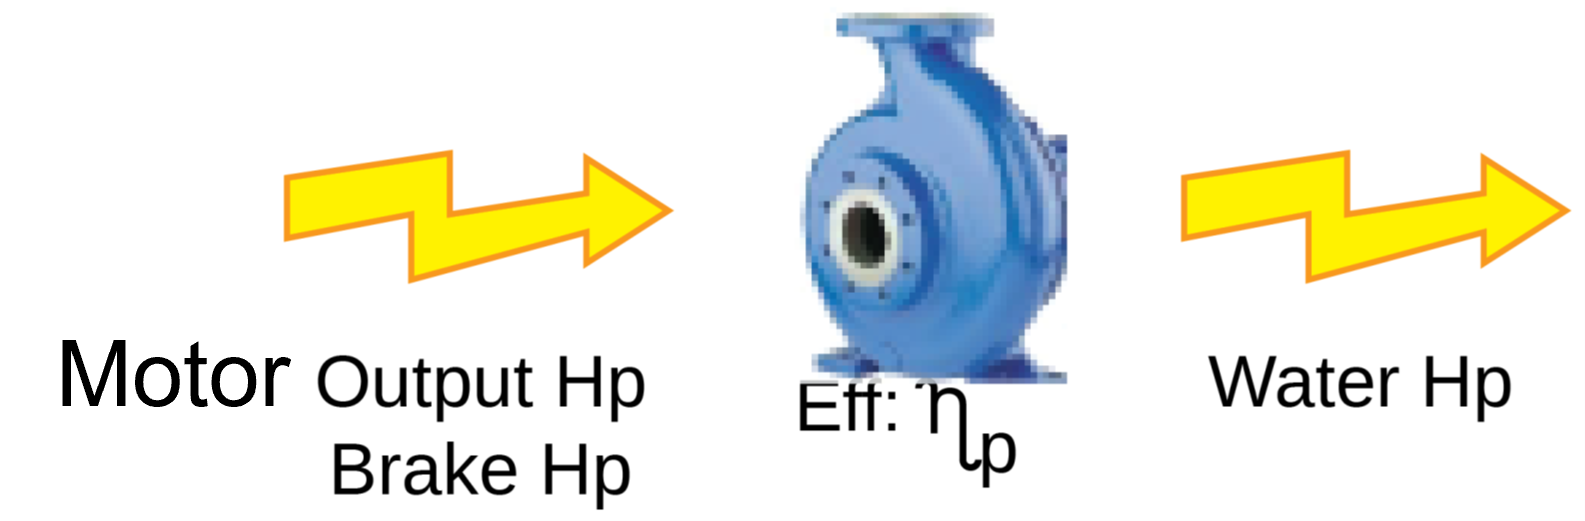
\includegraphics[scale=0.32]{PumpingProblemPump}
 \vspace{0.2cm}

water Hp = flow * head\\
 \vspace{0.2cm}
$\mathrm{Water} \enspace \mathrm{Hp} = 500 \enspace \mathrm{gpm}*50 \enspace ft*\dfrac{\mathrm{Hp}}{3,960 \enspace \mathrm{gpm-ft}}=\boxed{ 6.3 \enspace \mathrm{WHp}}$\\ 
  \vspace{0.2cm}
$\mathrm{Pump \enspace efficiency} =\dfrac{\mathrm{water \enspace Hp}}{\mathrm{brake \enspace Hp}} \implies \mathrm{brake \enspace Hp}=\dfrac{\mathrm{pump \enspace Hp}}{\mathrm{Pump \enspace efficiency}}$ \\
  \vspace{0.2cm}
$\textrm{brake} \enspace Hp = \dfrac{6.3}{0.85}=\boxed{7.4 \enspace \mathrm{Hp}}$\\
  \vspace{0.2cm}
$\mathrm{Motor \enspace efficiency} =\dfrac{\mathrm{brake \enspace Hp}}{\mathrm{input \enspace Hp}} \implies \mathrm{input \enspace \enspace Hp}=\dfrac{\mathrm{brake \enspace Hp}}{\mathrm{motor \enspace efficiency}}= \dfrac{7.4}{0.9}=\boxed{8.2 \enspace \mathrm{Hp}}$\\
  \vspace{0.2cm}
  
 \vspace{0.2cm}
$\mathrm{Wire-to-water} \enspace \mathrm{efficiency}=\eta_m * \eta_p \implies 0.9 \times 0.85 \times 100=\boxed{77 \%}$

  \item Find the brake horsepower for a pump given the following information: Total Dynamic Head $=75$ feet, Pump Rate $=150$ gpm, Pump Efficiency $=90 \%$, Motor Efficiency $=85 \%$\\
  
  Solution:\\
\vspace{0.4cm}
water Hp = flow * head\\
$150 \enspace \mathrm{GPM}*75\mathrm{ft}*\dfrac{Hp}{3,960 GPM-ft}=\boxed{Water \enspace Hp = 2.8Hp}$\\
\vspace{0.4cm}
pump Hp = brake Hp * pump efficiency\\
$brake \enspace Hp = \dfrac{2.8}{0.9}=\boxed{Brake \enspace Hp=3.1Hp}$
 \vspace{0.2cm}

\item The water horsepower of a pump is $10 \mathrm{Hp}$ and the brake horsepower output of the motor is $15.4 \mathrm{Hp}$. What is the efficiency of the pump?\\
\vspace{0.2cm}
Solution:\\ 
 \vspace{0.2cm}
 \vspace{0.4cm}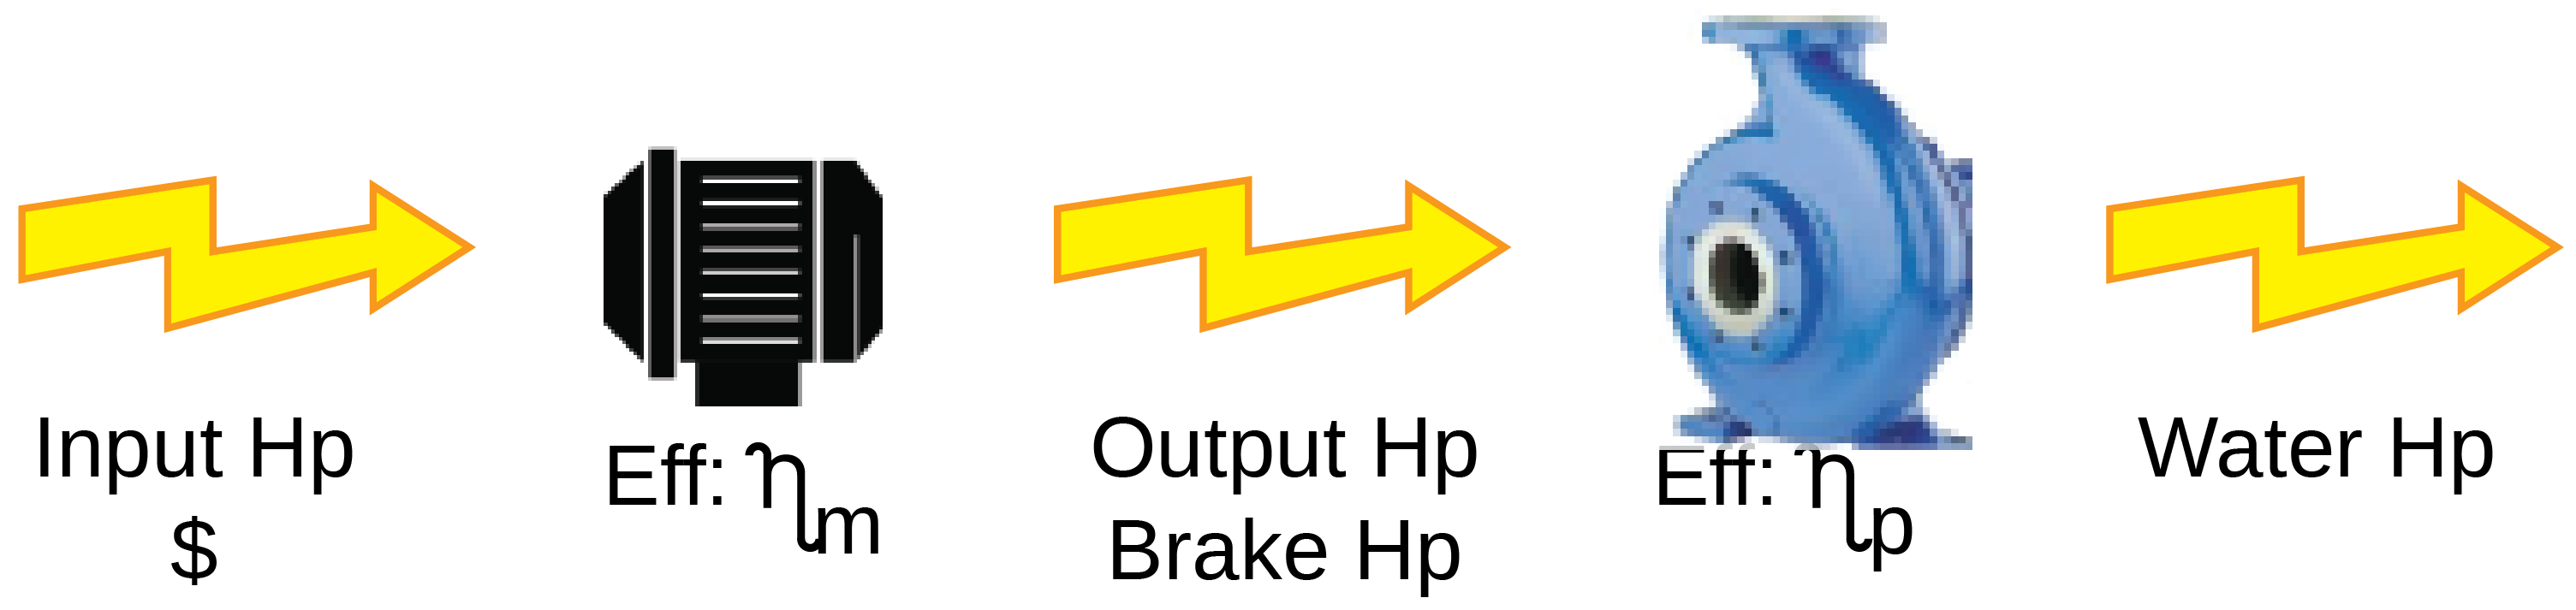
\includegraphics[scale=0.08]{PumpProblem}\\
 \vspace{0.2cm}
 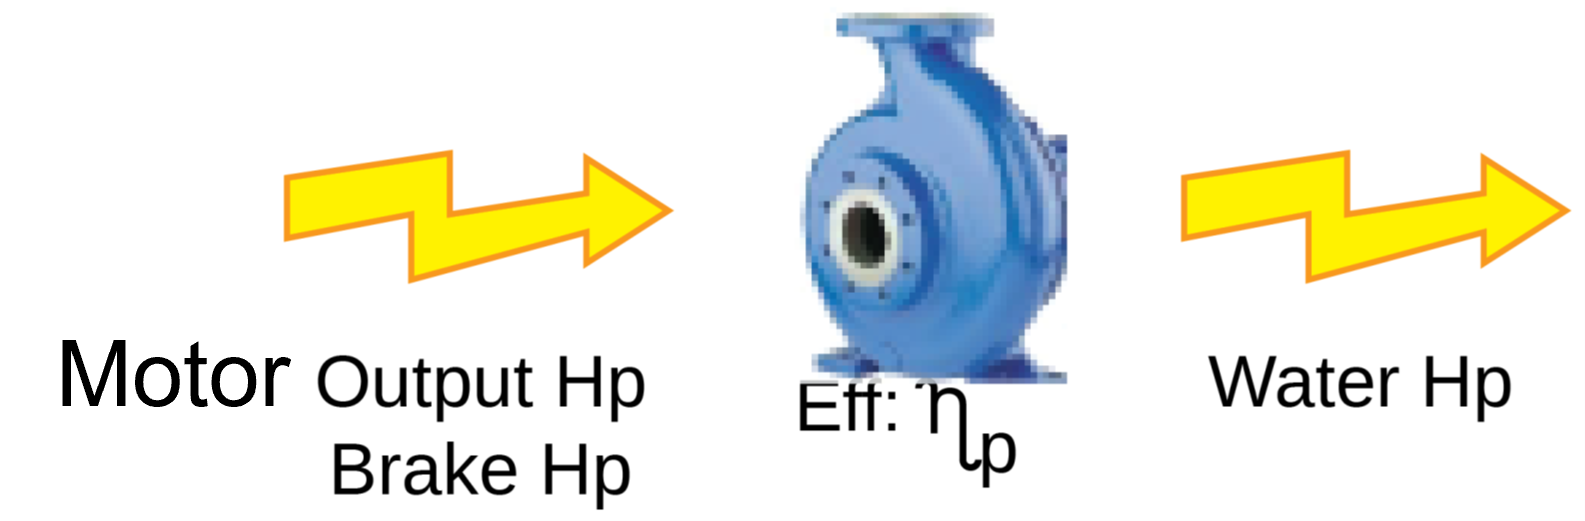
\includegraphics[scale=0.32]{PumpingProblemPump}
 $\eta_p=\dfrac{10 \mathrm{BHp}}{15.4 \mathrm{EHp}} \times 100=\boxed{65 \%}$\\
 \vspace{0.2cm}
 \item The water horsepower of a pump is $25 \mathrm{Hp}$ and the brake horsepower output of the motor is $48 \mathrm{Hp}$. What is the efficiency of the pump?\\
 Solution:\\
  \vspace{0.2cm}
 \vspace{0.32cm}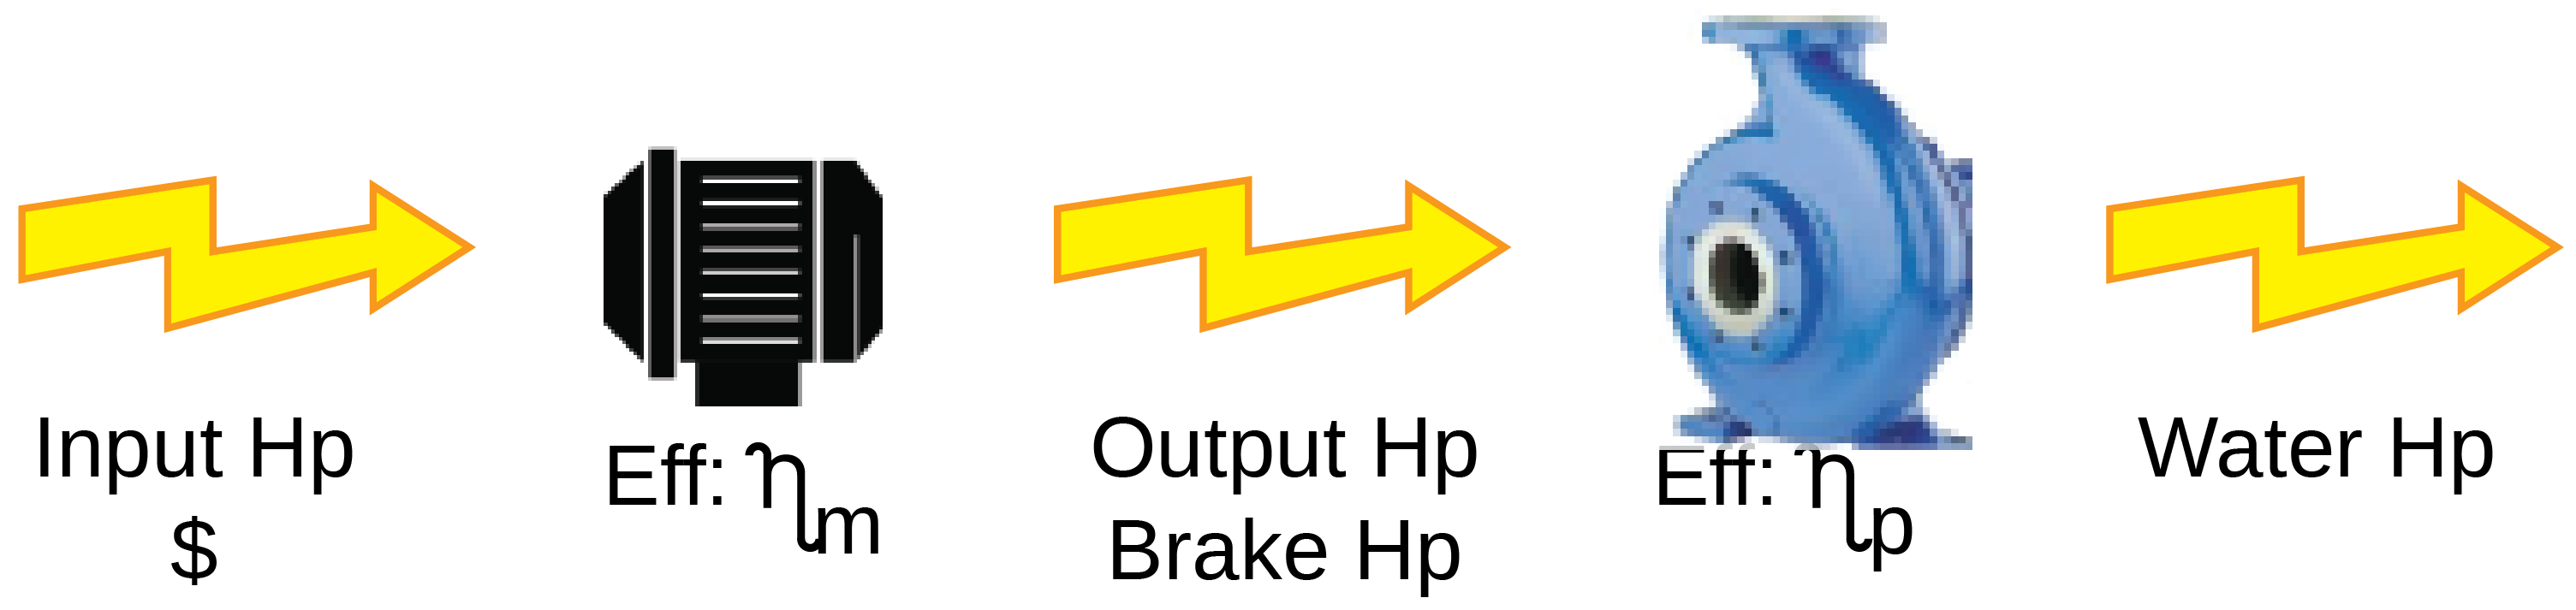
\includegraphics[scale=0.08]{PumpProblem}\\
 \vspace{0.2cm}
 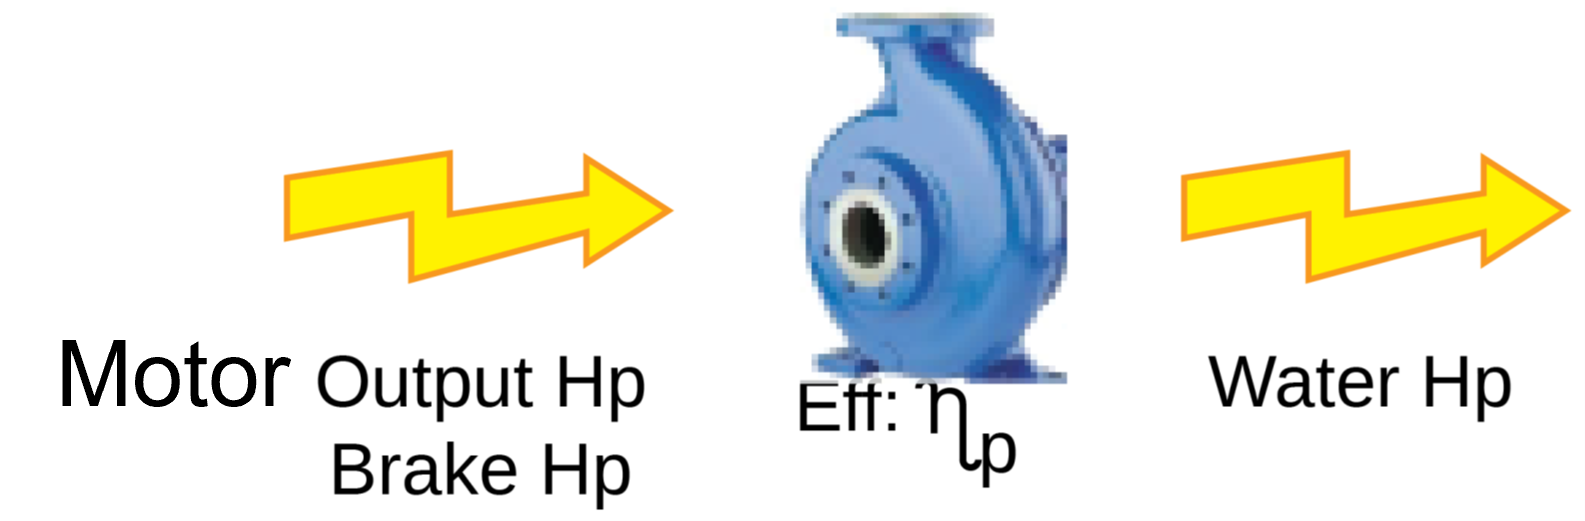
\includegraphics[scale=0.4]{PumpingProblemPump}
 \vspace{0.2cm}
$\eta_p=\dfrac{25 \mathrm{\enspace Water \enspace Hp}}{48 \mathrm{\enspace brake \enspace Hp}} \times 100=\boxed{52 \%}$
  \vspace{0.4cm}
  
  
  


\item The efficiency of a well pump is determined to be $75 \%$. The efficiency of the motor is estimated at $94 \%$. What is the efficiency of the well?\\
 \vspace{0.2cm}
Solution:\\ 
 \vspace{0.2cm}
$Well \enspace efficiency=\eta_m * \eta_p \implies 0.94 \times 0.75=0.705 \times 100=\boxed{71 \%}$
 \vspace{0.2cm}

  \item Water is being pumped from a reservoir to a storage tank on a hill. The elevation difference between water levels is 1200 feet. Find the pump size (in Hp) required to fill the tank at a rate of 120 gpm.\\
  \vspace{0.2cm}
\begin{tikzpicture}[scale=1]
\draw (0,0) .. controls (1.98,3.5) and (2.02,3.5) .. (4,0);
\node[cylinder, 
    draw = violet, 
    text = purple,
    cylinder uses custom fill, 
    cylinder body fill = blue!10, 
    cylinder end fill = magenta!40,
    aspect = 0.1, 
    shape border rotate = 90] (c) at (2,3.0) {Storage};
\node[cylinder, 
    draw = violet, 
    text = purple,
    cylinder uses custom fill, 
    %cylinder body fill = magenta!10, 
    %cylinder end fill = magenta!40,
    minimum size = 0.3cm, aspect = 0.1,
    shape border rotate = 90] (c) at (2,3.5) {\hspace{0.25cm}{Water}\hspace{0.25cm}};

  \node at (-3,0.1) {\includegraphics[width=3cm]{PumpIcon.png}};
   \node at (-3,-0.8) {
\includegraphics[width=2cm]{WaterReservoirIcon.png}};
   
\draw [ultra thick, -] (-3,-.9) -- (-3,0) node [midway, below] {};
\draw [ultra thick, -] (-3.28,0.63) -- (-3.28,3.1) node [midway, below] {};
\draw [ultra thick, ->] (-3.28,3.1) -- (1.2,3.1) node [midway, below] {};
\draw [ultra thick, ->] (-3.28,3.1) -- (1.2,3.1) node [midway, below] {};
\draw[dashed] (-1.8,-1) -- (2.5,-1);
\draw [<->] (2,-1) -- (2,3.25) node [midway, below] {\hspace{5cm}Elevation difference = 1200 ft};
\draw (0.5,3.7) node[anchor=north east] {$Flow = 120 gpm$};
\end{tikzpicture}\\
\vspace{0.2cm}
Solution:\\
\vspace{0.2cm}
water Hp = flow * head\\
$120GPM*1,200ft*\dfrac{Hp}{3,960 GPM-ft}=\boxed{Water \enspace Hp = 36.4Hp}$\\
\item If a pump is operating at 2,200 gpm and 60 feet of head, what is the water horsepower? If the pump efficiency is 71\%, what is the brake horsepower?\\
\vspace{0.2cm}
Solution:\\
\vspace{0.2cm}
water Hp = flow * head\\
$2,200GPM*60ft*\dfrac{Hp}{3,960 GPM-ft}=\boxed{Water \enspace Hp = 33.3Hp}$\\
\vspace{0.4cm}
pump Hp = brake Hp * pump efficiency\\
$brake \enspace Hp = \dfrac{33.3}{0.71}=\boxed{Brake \enspace Hp=47Hp}$
 \vspace{0.2cm}


\item The water horsepower of a pump is $10 \mathrm{Hp}$ and the brake horsepower output of the motor is $15.4 \mathrm{Hp}$. What is the efficiency of the pump?\\
\vspace{0.2cm}
Solution:\\ 
 \vspace{0.2cm}
 \vspace{0.4cm}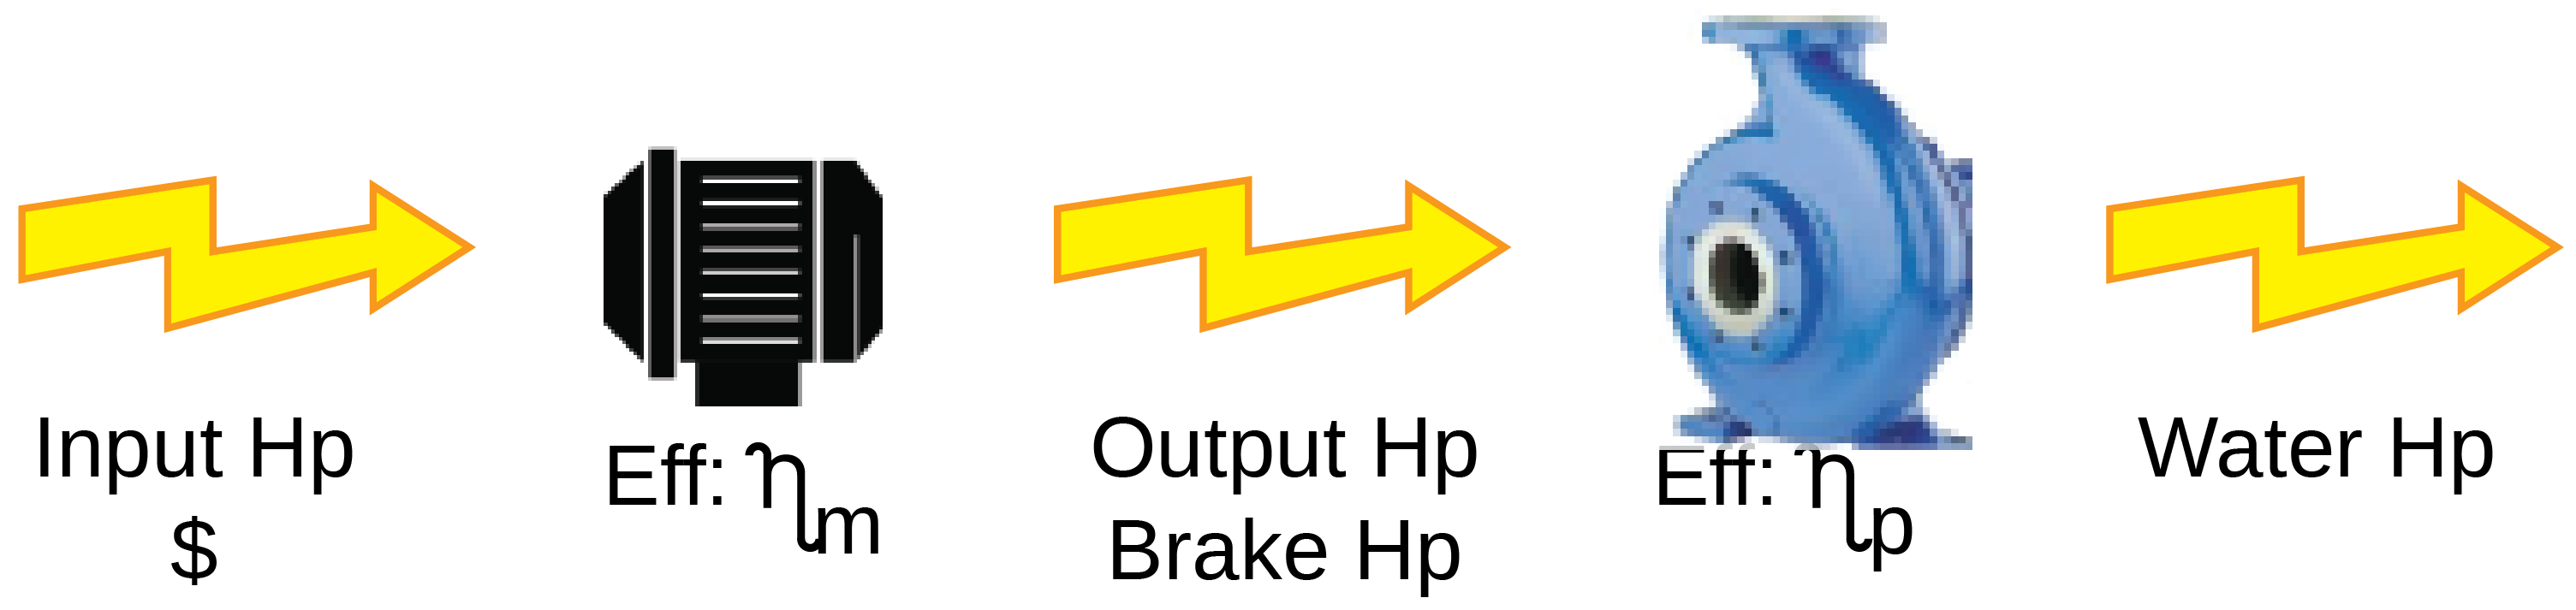
\includegraphics[scale=0.08]{PumpProblem}\\
 \vspace{0.2cm}
 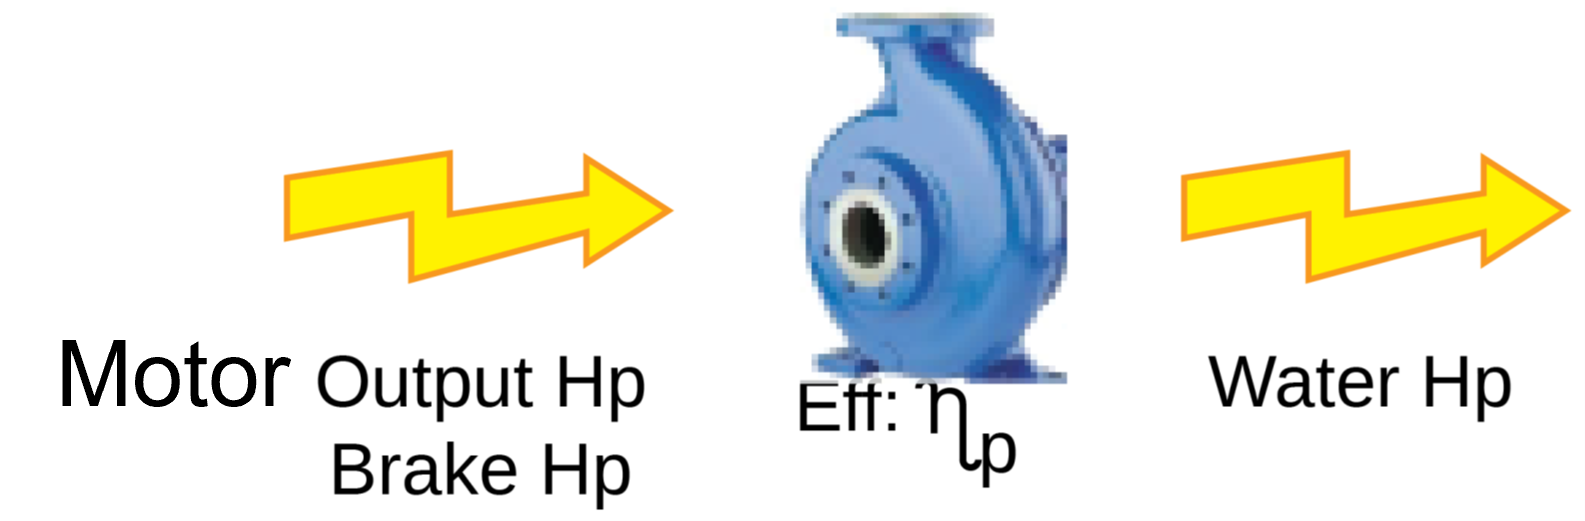
\includegraphics[scale=0.32]{PumpingProblemPump}
 $\eta_p=\dfrac{10 \mathrm{BHp}}{15.4 \mathrm{EHp}} \times 100=\boxed{65 \%}$\\
 \vspace{0.2cm}
 \item The water horsepower of a pump is $25 \mathrm{Hp}$ and the brake horsepower output of the motor is $48 \mathrm{Hp}$. What is the efficiency of the pump?\\
 Solution:\\
  \vspace{0.2cm}
 \vspace{0.32cm}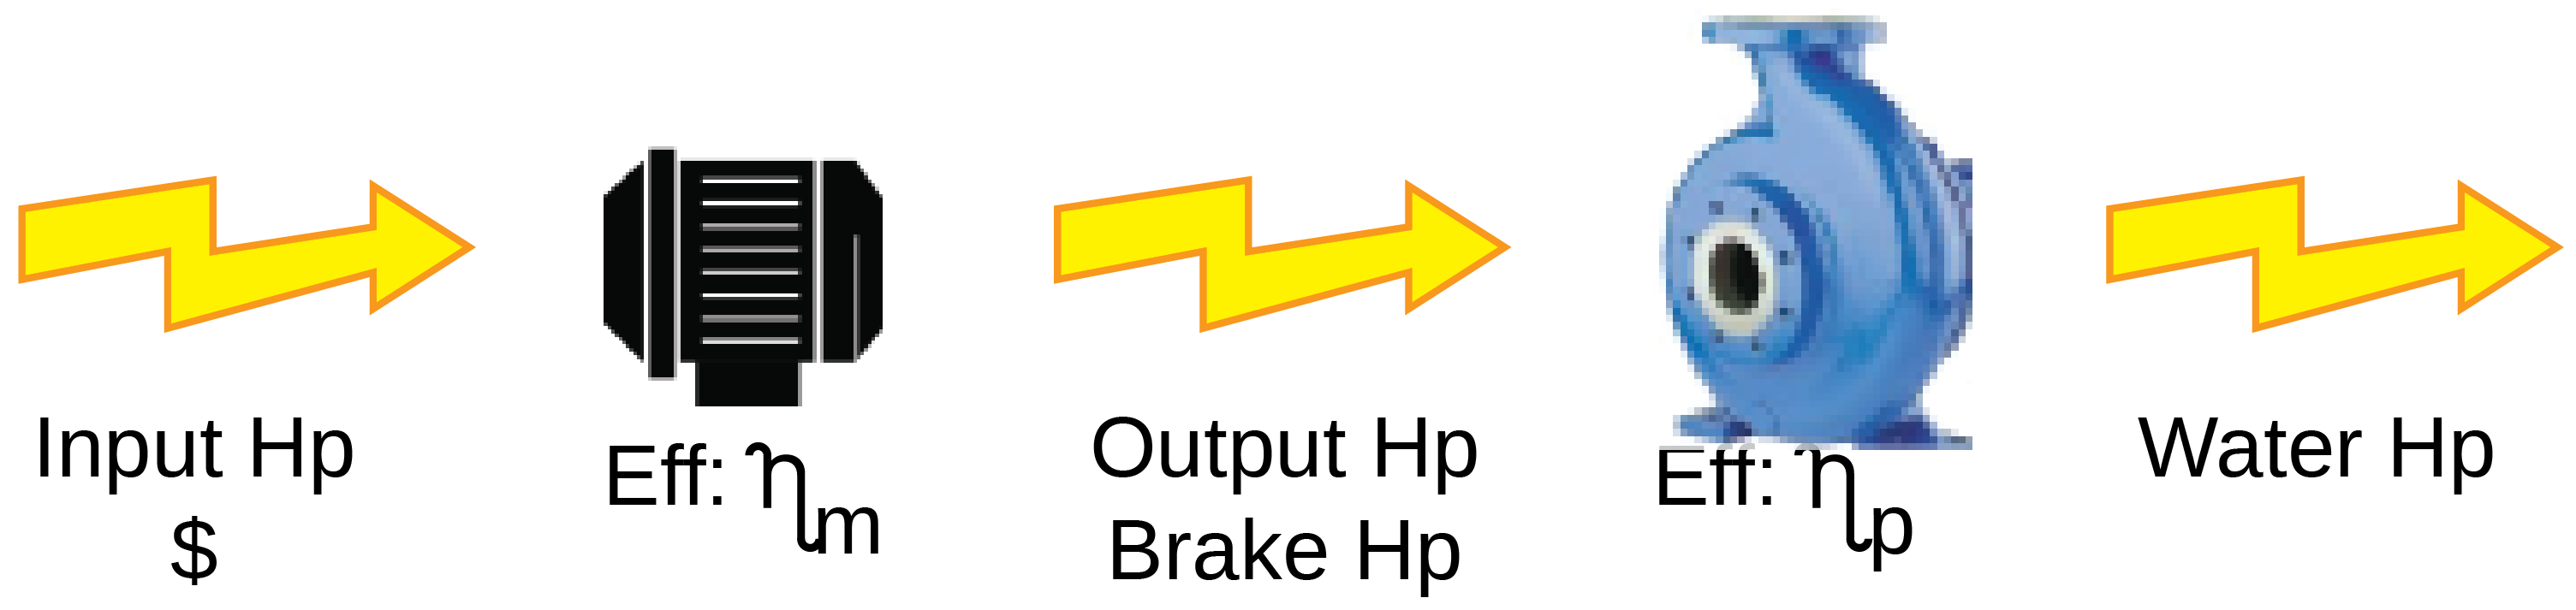
\includegraphics[scale=0.08]{PumpProblem}\\
 \vspace{0.2cm}
 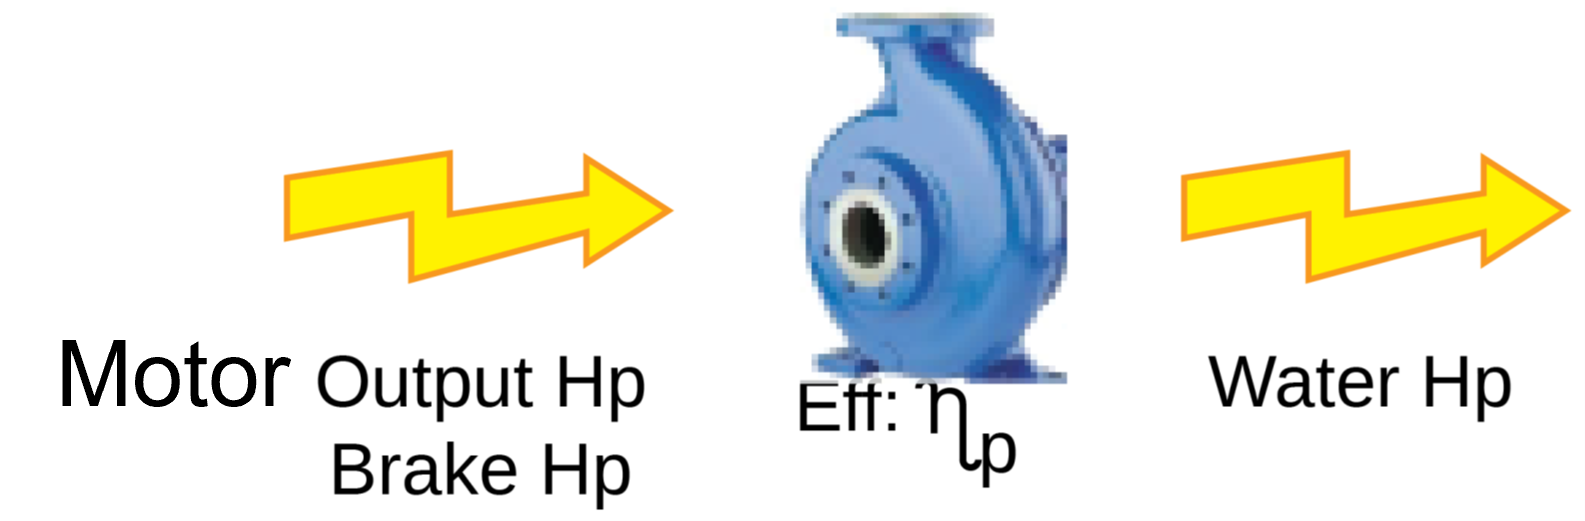
\includegraphics[scale=0.4]{PumpingProblemPump}
 \vspace{0.2cm}
$\eta_p=\dfrac{25 \mathrm{\enspace Water \enspace Hp}}{48 \mathrm{\enspace brake \enspace Hp}} \times 100=\boxed{52 \%}$
  \vspace{0.4cm}
  
  

\item The efficiency of a well pump is determined to be $75 \%$. The efficiency of the motor is estimated at $94 \%$. What is the efficiency of the well?\\
 \vspace{0.2cm}
Solution:\\ 
 \vspace{0.2cm}
$Well \enspace efficiency=\eta_m * \eta_p \implies 0.94 \times 0.75=0.705 \times 100=\boxed{71 \%}$
 \vspace{0.2cm}

  \item Water is being pumped from a reservoir to a storage tank on a hill. The elevation difference between water levels is 1200 feet. Find the pump size (in Hp) required to fill the tank at a rate of 120 gpm.\\
  \vspace{0.2cm}
\begin{tikzpicture}[scale=1]
\draw (0,0) .. controls (1.98,3.5) and (2.02,3.5) .. (4,0);
\node[cylinder, 
    draw = violet, 
    text = purple,
    cylinder uses custom fill, 
    cylinder body fill = blue!10, 
    cylinder end fill = magenta!40,
    aspect = 0.1, 
    shape border rotate = 90] (c) at (2,3.0) {Storage};
\node[cylinder, 
    draw = violet, 
    text = purple,
    cylinder uses custom fill, 
    %cylinder body fill = magenta!10, 
    %cylinder end fill = magenta!40,
    minimum size = 0.3cm, aspect = 0.1,
    shape border rotate = 90] (c) at (2,3.5) {\hspace{0.25cm}{Water}\hspace{0.25cm}};

  \node at (-3,0.1) {\includegraphics[width=3cm]{PumpIcon.png}};
   \node at (-3,-0.8) {
\includegraphics[width=2cm]{WaterReservoirIcon.png}};
   
\draw [ultra thick, -] (-3,-.9) -- (-3,0) node [midway, below] {};
\draw [ultra thick, -] (-3.28,0.63) -- (-3.28,3.1) node [midway, below] {};
\draw [ultra thick, ->] (-3.28,3.1) -- (1.2,3.1) node [midway, below] {};
\draw [ultra thick, ->] (-3.28,3.1) -- (1.2,3.1) node [midway, below] {};
\draw[dashed] (-1.8,-1) -- (2.5,-1);
\draw [<->] (2,-1) -- (2,3.25) node [midway, below] {\hspace{5cm}Elevation difference = 1200 ft};
\draw (0.5,3.7) node[anchor=north east] {$Flow = 120 gpm$};
\end{tikzpicture}\\
\vspace{0.2cm}
Solution:\\
\vspace{0.2cm}
water Hp = flow * head\\
$120GPM*1,200ft*\dfrac{Hp}{3,960 GPM-ft}=\boxed{Water \enspace Hp = 36.4Hp}$\\
\item If a pump is operating at 2,200 gpm and 60 feet of head, what is the water horsepower? If the pump efficiency is 71\%, what is the brake horsepower?\\
\vspace{0.2cm}
Solution:\\
\vspace{0.2cm}
water Hp = flow * head\\
$2,200GPM*60ft*\dfrac{Hp}{3,960 GPM-ft}=\boxed{Water \enspace Hp = 33.3Hp}$\\
\vspace{0.4cm}
pump Hp = brake Hp * pump efficiency\\
$brake \enspace Hp = \dfrac{33.3}{0.71}=\boxed{Brake \enspace Hp=47Hp}$
 \vspace{0.2cm}


\item The water horsepower of a pump is $10 \mathrm{Hp}$ and the brake horsepower output of the motor is $15.4 \mathrm{Hp}$. What is the efficiency of the pump?\\
\vspace{0.2cm}
Solution:\\ 
 \vspace{0.2cm}
 \vspace{0.4cm}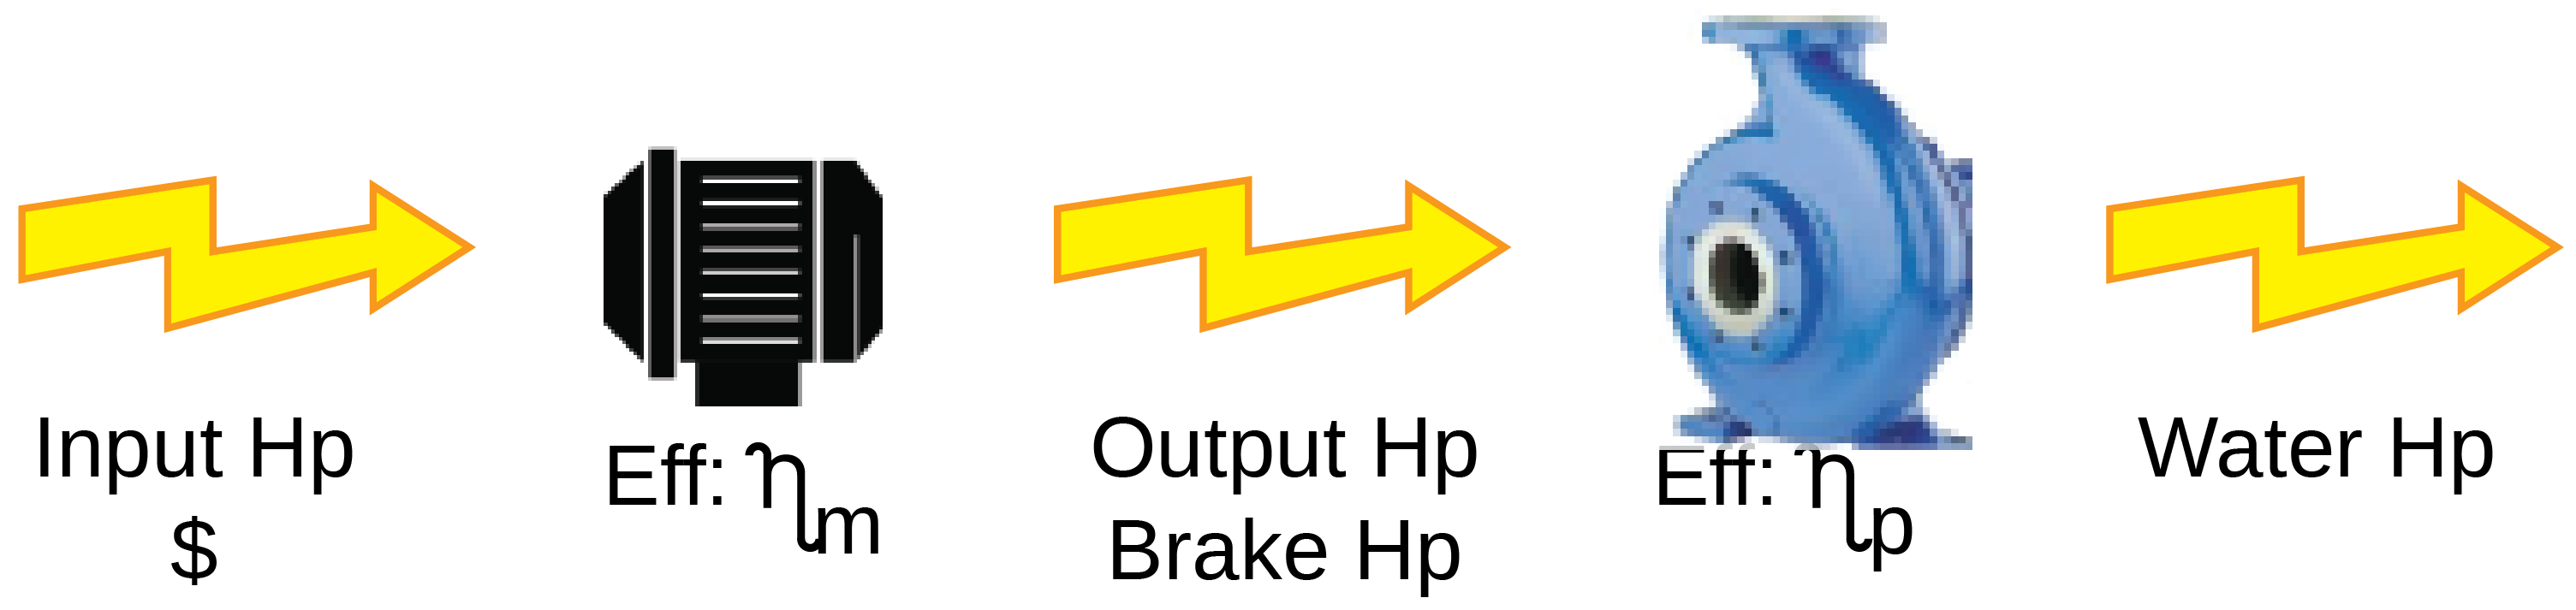
\includegraphics[scale=0.08]{PumpProblem}\\
 \vspace{0.2cm}
 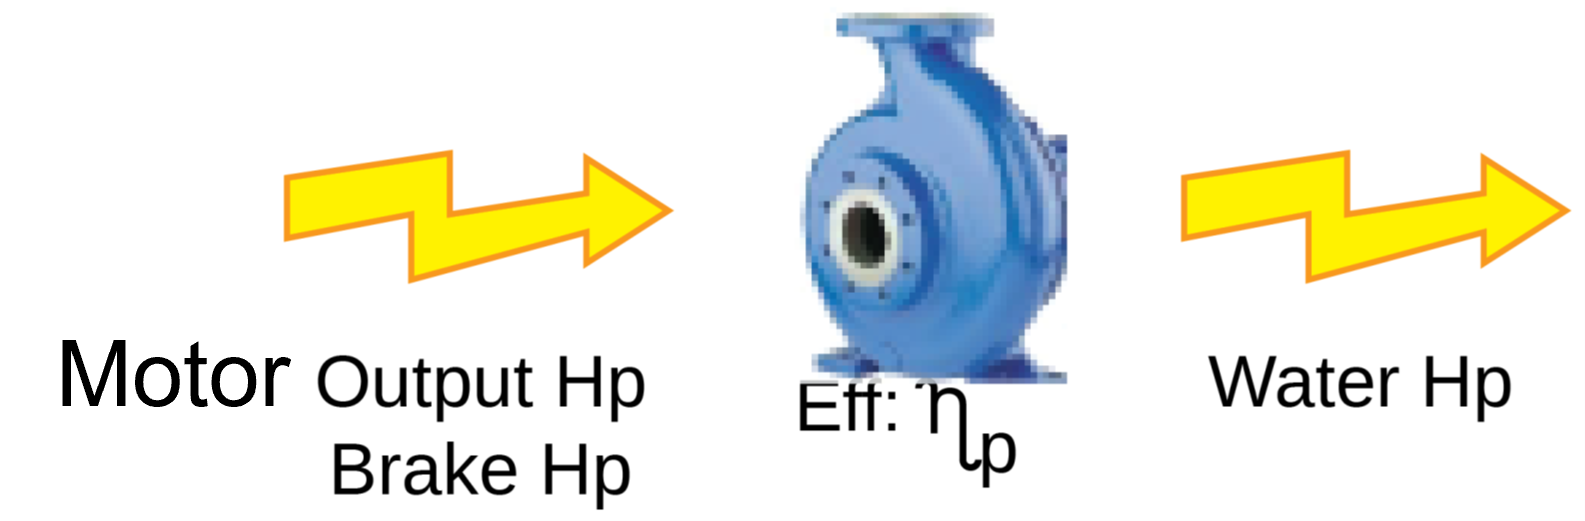
\includegraphics[scale=0.32]{PumpingProblemPump}
 $\eta_p=\dfrac{10 \mathrm{BHp}}{15.4 \mathrm{EHp}} \times 100=\boxed{65 \%}$\\
 \vspace{0.2cm}
 \item The water horsepower of a pump is $25 \mathrm{Hp}$ and the brake horsepower output of the motor is $48 \mathrm{Hp}$. What is the efficiency of the pump?\\
 Solution:\\
  \vspace{0.2cm}
 \vspace{0.32cm}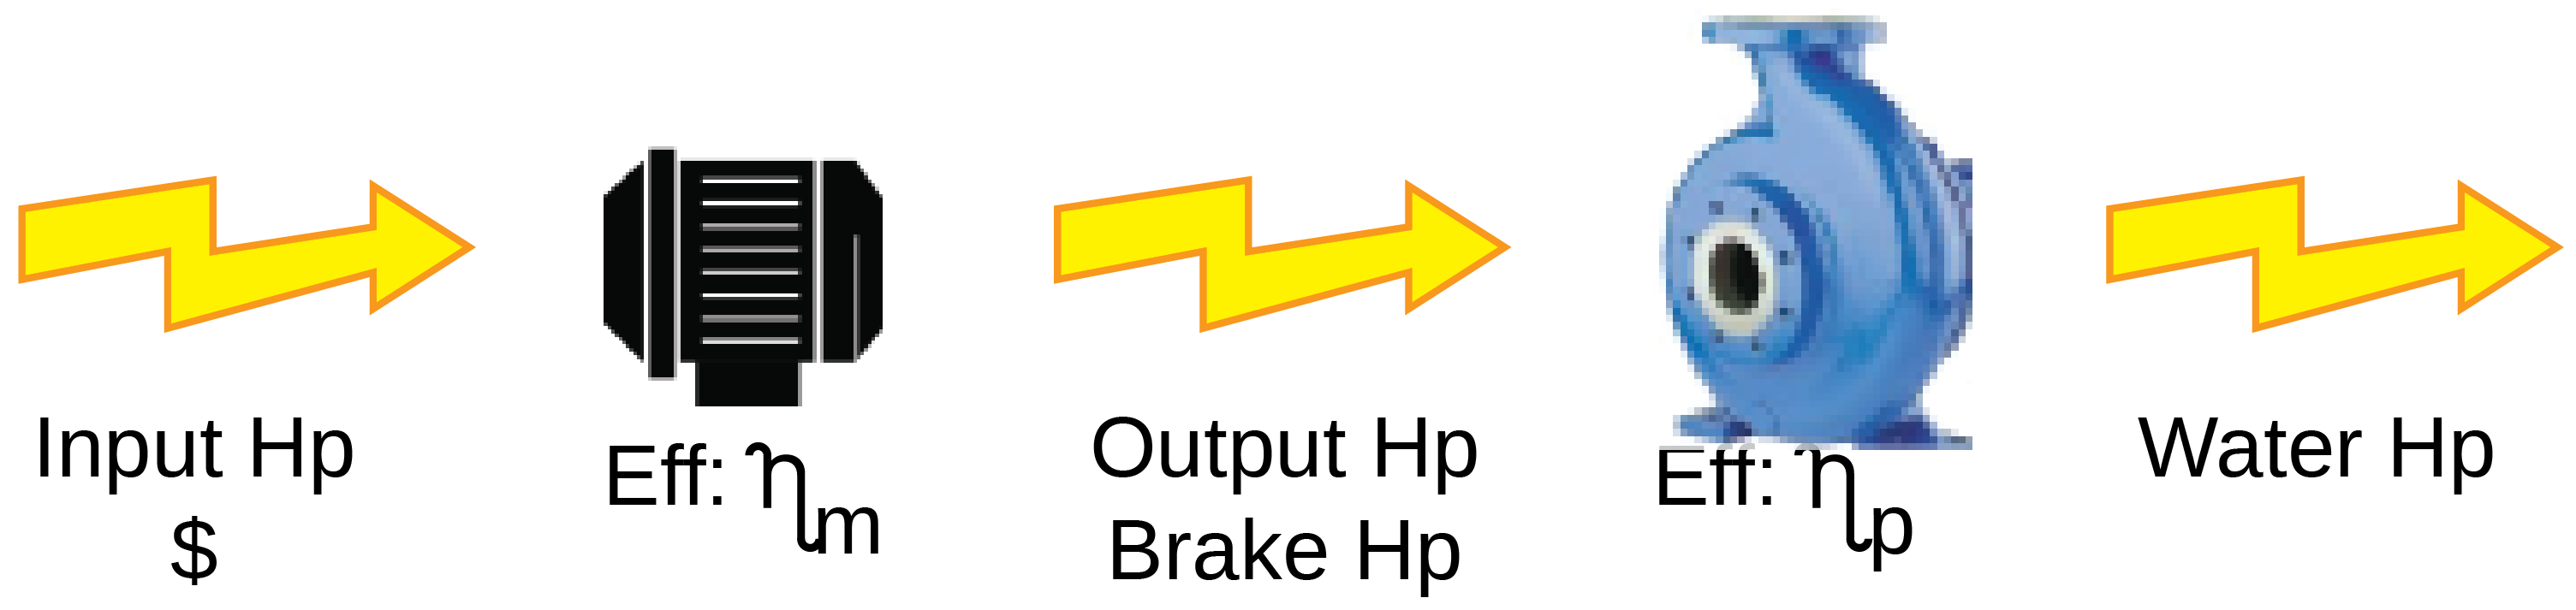
\includegraphics[scale=0.08]{PumpProblem}\\
 \vspace{0.2cm}
 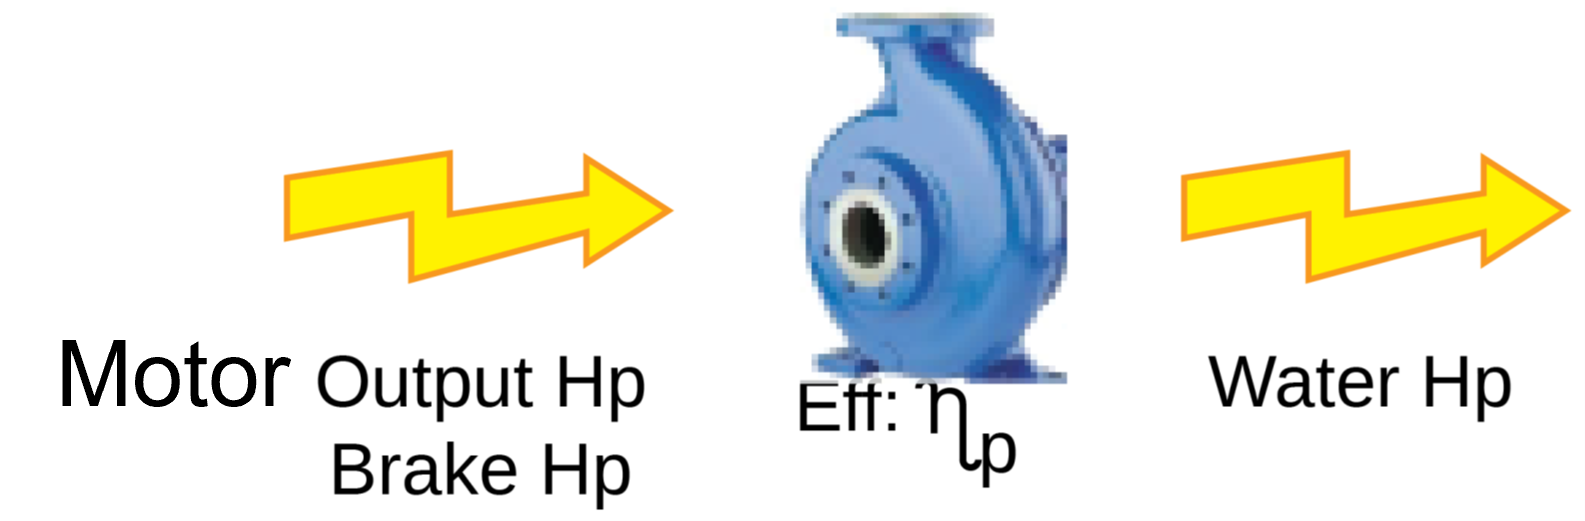
\includegraphics[scale=0.4]{PumpingProblemPump}
 \vspace{0.2cm}
$\eta_p=\dfrac{25 \mathrm{\enspace Water \enspace Hp}}{48 \mathrm{\enspace brake \enspace Hp}} \times 100=\boxed{52 \%}$
  \vspace{0.4cm}
  
  
\item A 240 volt motor runs an average of 8 hours a day.  If the electric meter registered 6,450 kilowatt hours for a 31-day month, what is the motor horsepower? [35 Hp]




\item A pump is equipped with a pressure gauge in the discharge pipe that reads 100 psi. The total discharge head in feet would be?\\
\vspace{0.4cm}
$100psi*\frac{2.31ft \enspace water}{psi}=\boxed{231ft \enspace water}$
\vspace{0.4cm}

\vspace{0.4cm}
\item 900 GPM pump is pumped against a 12 ft head.  What is the water Hp
\vspace{0.4cm}
water Hp = flow * head\\
$900GPM*12ft*\frac{Hp}{3,960 GPM-ft}=\boxed{2.7Hp}$

\item A 50 ft$^3$/sec flow is pumped against a head of 8 feet.  What is the water Hp

\vspace{0.4cm}
water Hp = flow * head\\
$\dfrac50{ft^3}{sec}*8ft*\frac{7.48 gal}{ft^3}*\frac{60sec}{min}*\frac{Hp}{3,960 GPM-ft}=\boxed{45.4Hp}$

\item 1 MGD is pumped against a 14’ head.  What is the water Hp?  The pump mechanical efficiency is 85\%.  What is the brake horsepower?\\
\vspace{0.4cm}
water Hp = flow * head\\
$\frac{1,000,000gal}{day}*\frac{day}{1440min}*14ft*\frac{Hp}{3,960 GPM-ft}=\boxed{Water \enspace Hp = 2.46Hp}$\\
\vspace{0.4cm}
pump Hp = brake Hp * pump efficiency\\
$brake \enspace Hp = \frac{2.46}{0.85}=\boxed{Brake \enspace Hp=2.89Hp}$


\item A flow of 2.5 MGD is being lifted 10 feet and then pumped up another 120 feet to a storage reservoir. Calculate the pump output power required to lift this water. Ignore friction losses.\\
\vspace{0.4cm}
water Hp = flow * head\\
$\frac{2,500,000gal}{day}*\frac{day}{1440min}*(120+10)ft*\frac{Hp}{3,960 GPM-ft}=\boxed{Water \enspace Hp = 57Hp}$\\
\pagebreak


\item A pump is pumping 400 gpm.  The suction pressure gauge indicates a pressure of 5 ft and the pump discharge pressure gauge indicates a pressure of 100 ft.  If the pump brake horse power is 12 hp, what is the pump efficiency\\
\vspace{0.4cm}
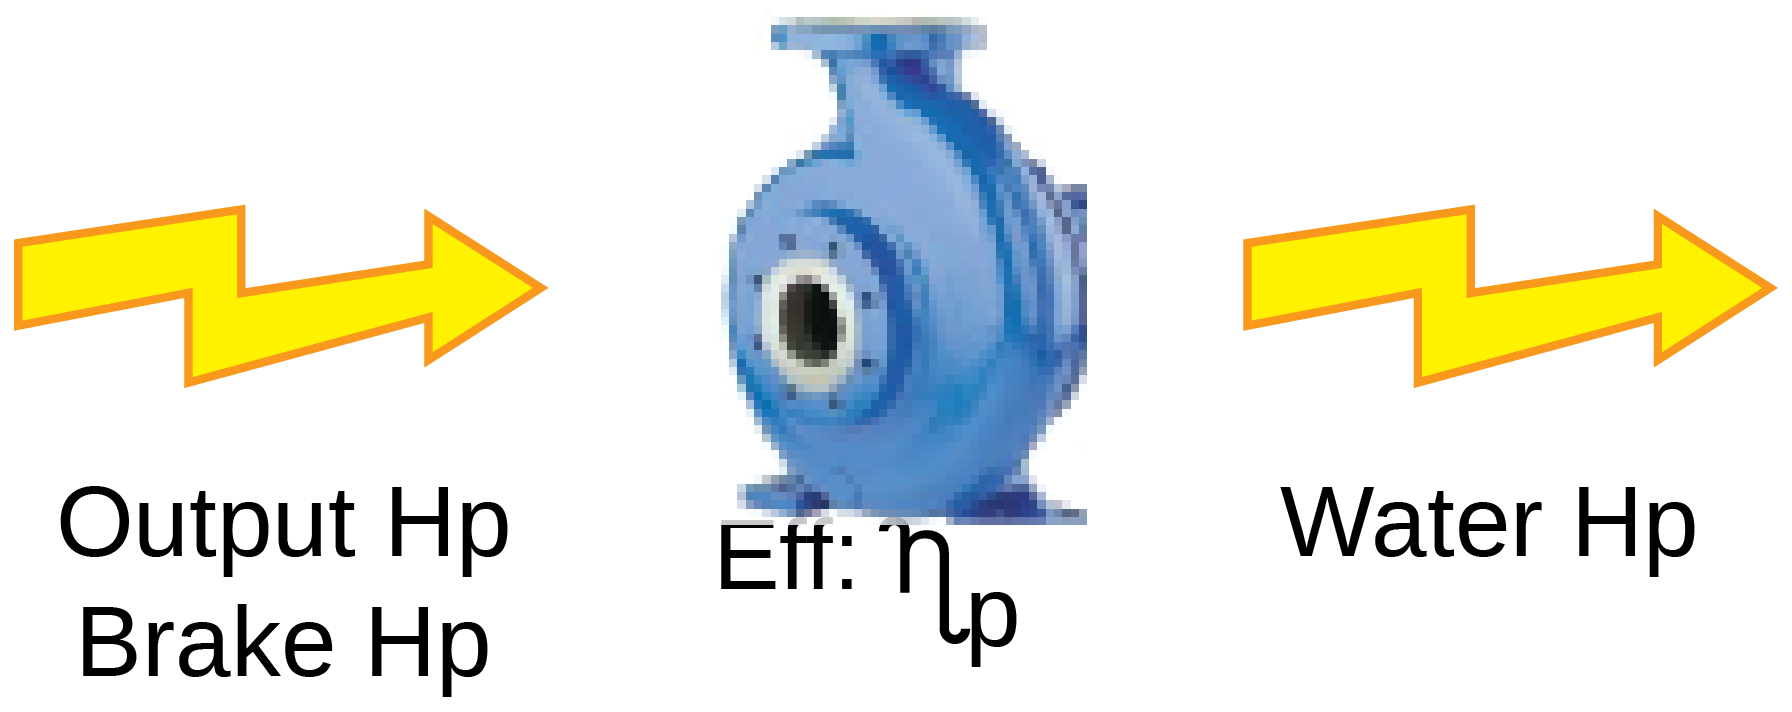
\includegraphics[scale=0.08]{PumpProblemPumpHp}\\
water Hp = flow * head\\
$400gpm*(100-5)ft*\frac{Hp}{3,960 gpm-ft}=\boxed{9.6Hp}$\\
\vspace{0.4cm}
pump efficiency - $\eta_p$=$\frac{9.6Hp}{12Hp}*100=\boxed{79\%}$
\vspace{0.4cm}

\item A flow of 200 gpm  is pumped against a total head of 4.0 feet. · The pump is 78\% efficient and the motor' is 90\% efficient. Calculate the input Hp.\\
\vspace{0.4cm}
water Hp = flow * head\\
$200GPM*4ft*\frac{Hp}{3,960 GPM-ft}=0.2Hp$\\
\vspace{0.4cm}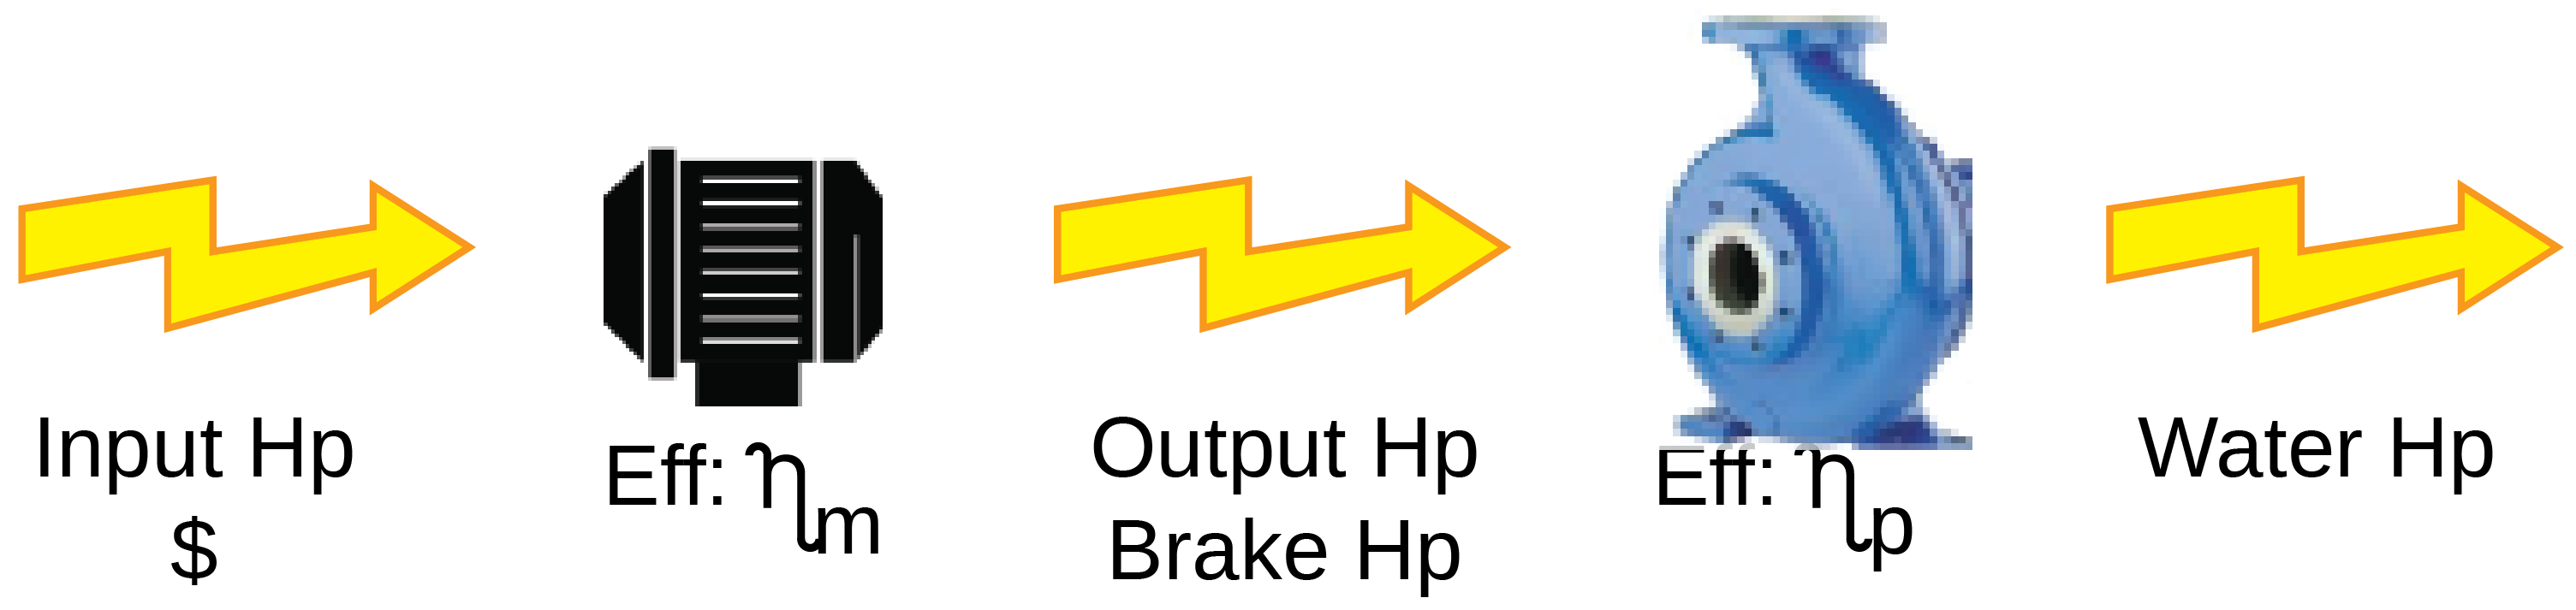
\includegraphics[scale=0.08]{PumpProblem}\\
water Hp=brake Hp*pump efficiency, and\\
brake Hp=input Hp*motor efficiency\\
Therefore, water Hp=input Hp*motor efficiency*pump efficiency\\
\vspace{0.4cm}
input Hp=$\frac{water \enspace Hp}{motor \enspace efficiency*pump \enspace efficiency}=\frac{0.2}{0.9*0.78}=\boxed{0.28Hp}$

\pagebreak

\item 500,000 gpd of secondary· effluent is pumped to  a  storage  pond  for  reuse  as golf course irrigation water.  The water is lifted 12 feet in the plant, and then pumped up another 75 feet to the storage pond. Friction losses are assumed to be 10\% of the static head.  Assuming the pump efficiency of 70\% and a motor efficiency of 92\% and an electrical cost of \$0.0725 per KWh, calculate the daily cost of pumping this water.\\
\vspace{0.4cm}
Solution:\\

water Hp = flow * head\\
\vspace{0.4cm}
$\frac{500,000gal}{day}*\frac{day}{1440min}*(87ft-static \enspace head+87*0.1ft-friction \enspace head)*\frac{Hp}{3,960 GPM-ft}$\\
$=8.39 - water \enspace Hp$\\
\vspace{0.4cm}
input Hp=$\frac{water \enspace Hp}{motor \enspace efficiency*pump \enspace efficiency}=\frac{8.39}{0.92*0.70}=\boxed{13Hp}$\\
\vspace{0.4cm}
Electrical cost=$13Hp*\frac{0.746kW}{Hp}*\frac{24hrs}{day}*\frac{\$0.0725}{kWh}=\boxed{\frac{\$16.87}{day}}$

\vspace{0.4cm}


\item A pump motor (93\% efficient) generates an output of 130 HP and runs 75\% of the time. Electricity costs an average of 8.455 cents per kilowatt-hour. What is the monthly cost of operating this pump in \$ per month?\\
\vspace{0.4cm}
$\frac{130Hp}{0.93}*\frac{0.746kW}{Hp}*\frac{24hrs}{day}*\frac{30days}{month}*0.75*\frac{\$0.08455}{kWh}=\boxed{\frac{\$4,761}{month}}$
\pagebreak


\item A wet well is 8 ft x 8 ft x 16.5 ft deep and receives a continuous flow of 310,000 gpd.  A 500 gpm pump draws down 12 feet of water each pumping cycle.  The motor that drives the pump draws 52.5 Hp when it pumps.  The cost of electricity is \$0.0755 per kilowatt - hour.  Calculate\\ 
(a) the time it takes to pump down the wet well, and\\
(b) The daily electrical energy cost for this pump.\\


\vspace{0.4cm}
Solution:\\
@$\frac{310,000gal}{day}*\frac{day}{1440min}=\frac{215.3gal}{min}$\\
\vspace{0.4cm}
Volume of wetwell that will be pumped down with the 500 gpm pump and a 215.3 gpm flow to the wetwell:\\
$\frac{500gal}{min}-\frac{215.3gal}{min}=\frac{284.7gal}{min}$\\
\vspace{0.4cm}
Minutes required to pump down the wetwell :\\
$8*8*12ft^3*\frac{7.48gal}{ft^3}*\frac{min}{284.7gal}=\boxed{20.2min}$\\
\vspace{0.4cm}
Time to fill wetwell with pump off @215.3gal/min influent flow:
\\
$8*8*12ft^3*\frac{7.48gal}{ft^3}*\frac{min}{215.3gal}=26.7min$\\
\vspace{0.4cm}
\# of cycles per day:\\
$\frac{cycle}{(20.2+26.7)min}*\frac{1440min}{day}=\frac{30.7cycles}{day}$\\
\vspace{0.4cm}
\# of hrs pump operational:\\
$\frac{20.2min}{cycle}*\frac{30.7 cycles}{day}*\frac{hrs}{60min}=\frac{10.33hours}{day}$\\
\vspace{0.4cm}
Daily electrical cost:\\
$52.5Hp*\frac{0.746kW}{Hp}*\frac{10.33hrs}{day}*\frac{\$0.0755}{kWh}=\boxed{\frac{\$30.54}{day}}$\\
\pagebreak


\item A 6-year old pump motor is to be replaced at a net cost of \$15,800. The new motor, just like the old one, would run 65\% of the time. Both existing and replacement motors would operate at 125 output Hp. The existing motor efficiency is 86\% while the replacement motor would be guaranteed at 94\% efficiency. Electricity currently averages \$0.088 per kWh.\\
(a) Calculate the energy cost savings per year (to the nearest dollar) if the existing motor is replaced with the new motor (neglect any consideration of impact upon demand charges or interest on capital).\\ (b) What is payback period to the nearest tenth of a year.
\vspace{0.4cm}
Energy cost savings per year:\\
Input Hp for old motor:$\frac{125}{0.86}=145.35Hp$\\
Input Hp for old motor:$\frac{125}{0.94}=132.98Hp$\\
Energy cost savings:\\$(145.35-132.98)Hp*\frac{0.746kW}{Hp}*\frac{(365*24*0.65)hrs}{yr}*\frac{\$0.088}{kWh}=\boxed{\frac{\$4,623.94}{yr}}$\\
\vspace{0.4cm}
Calculate payback:\\
$\$15,800*\frac{yr}{\$4,623.94}=\boxed{3.4yr}$

\item A 8 ft diameter cylindrical wetwell receives an average incoming flow if 135 gpm and is pumped down with a pump that delivers 450 gpm again a total dynamic head of 120 ft.  The pump is controlled using two floats; a stop float located at 2.5 ft and a start float located at 16 ft.  If the pump motor is rated at 88\% and the pump at 77\%, what is the monthly (30 days/month) for running this pump if power costs are \$0.11/Kwh?\\
\vspace{0.6cm}

 (Ans:  \$356/month)


\vspace{0.4cm}
Volume of wetwell that will be pumped down with the 450 gpm pump and a 135 gpm flow to the wetwell:\\
$\frac{450gal}{min}-\frac{135gal}{min}=\frac{315gal}{min}$\\
\vspace{0.4cm}
Minutes required to pump down the wetwell :\\
$0.785*8^2*(16-2.5)ft^3*\frac{7.48gal}{ft^3}*\frac{min}{315gal}=\boxed{16.1min}$\\
\vspace{0.4cm}
Time to fill wetwell with pump off @135gal/min influent flow:
\\
$[0.785*8^2*(16-2.5)]ft^3*\frac{7.48gal}{ft^3}*\frac{min}{135gal}=37.6min$\\
\vspace{0.4cm}
\# of cycles per day:\\
$\frac{cycle}{(16.1+37.6)min}*\frac{1440min}{day}=\frac{26.8cycles}{day}$\\
\vspace{0.4cm}
\# of hrs pump operational:\\
$\frac{16.1min}{cycle}*\frac{26.8 cycles}{day}*\frac{hrs}{60min}=\frac{7.19hours}{day}$\\
\vspace{0.4cm}
Daily electrical cost:\\
$\frac{450gpm*120ft}{0.88*0.77}*\frac{Hp}{3,960 gpm-ft}*\frac{0.746kW}{Hp}*\frac{7.19hrs}{day}*\frac{30days}{month}*\frac{\$0.11}{kWh}=\boxed{\frac{\$356}{day}}$\\
\vspace{1cm}


\item A pump operating at 80\% efficiency generates an water Hp of 60 HP and runs 75\% of the time. Assuming the pump motor is 90\% efficient and electricity costs an average of \$0.0821 per kilowatt-hour. Calculate the monthly (30 days) cost of operating this pump.\\
\vspace{0.4cm}
$\frac{60Hp}{0.90*0.80}*\frac{0.746kW}{Hp}*\frac{24hrs}{day}*\frac{30days}{month}*0.75*\frac{\$0.0821}{kWh}=\boxed{\frac{\$2,756}{month}} - Correct \enspace Answer$\\
$\frac{60Hp}{0.8}*\frac{0.746kW}{Hp}*\frac{24hrs}{day}*\frac{30days}{month}*0.75*\frac{\$0.0821}{kWh}=\boxed{\frac{\$2,480}{month}}$\\
$\frac{60Hp}{0.90}*\frac{0.746kW}{Hp}*\frac{24hrs}{day}*\frac{30days}{month}*0.75*\frac{\$0.0821}{kWh}=\boxed{\frac{\$2,205}{month}}$\\
$\frac{60Hp}{0.90*0.80}*\frac{0.746kW}{Hp}*\frac{24hrs}{day}*\frac{30days}{month}*\frac{\$0.0821}{kWh}=\boxed{\frac{\$3,675}{month}}$

\item A 8 ft diameter cylindrical wetwell receives an average incoming flow if 135 gpm and is pumped down with a pump that delivers 450 gpm again a total dynamic head of 120 ft. The pump is controlled using two floats; a stop float located at 2.5 ft and a start float located at 16 ft. If the pump motor is rated at 88\% and the pump at 77\%, what is the monthly (30 days/month) for running this pump if power costs are \$0.11/Kwh?\\
\vspace{0.6cm}



 (Ans: \$356/month) 

Correct Answer(s): 356.0\\
 


\item  A 8 ft diameter cylindrical wetwell receives an average incoming flow if 135 gpm and is pumped down with a pump that delivers 450 gpm again a total dynamic head of 120 ft. The pump is controlled using two floats; a stop float located at 2.5 ft and a start float located at 16 ft. If the pump motor is rated at 88\% and the pump at 77\%, what is the monthly (30 days/month) for running this pump if power costs are \$0.11/Kwh?\\
\vspace{0.6cm}



 (Ans: \$356/month)


Correct Answer(s): 

\item If a wasting pump has a fixed pump rate of 250 GPM, and your calculation
indicates you must waste 126,000 gallons, what hourly cycle rate do you set
the timer?\\
a. Turn pump on 21 minutes every day\\
b. Turn pump on 504 minutes every hour\\
c. Turn pump on 42 minutes every day\\
d. Turn pump on 21 minutes every hour\\

\vspace{0.3cm}
Solution:\\
\vspace{0.2cm}
$\frac{min}{hr}=\frac{126,000 \enspace gal}{day}*\frac{day}{24 \enspace hrs}*\frac{min}{250 \enspace gal}=\boxed{\frac{21 \enspace min}{hr}}$

\end{enumerate}
\end{document}